\documentclass[11pt]{amsart}

\def\npart{III}

\def\ntitle{Algebraic Number Theory Summary}
\def\nlecturer{Jack Throne}

\def\nterm{Michaelmas}
\def\nyear{2019}

\input{../preamble.tex}
\usepackage{wrapfig}
\usepackage{xcomment}

% \xcomment{prop,thm,lem,cor,defn}


% \newcommand{\sectionbreak}{\clearpage} % clear page after each section

% \surroundwithmdframed[style=leftbar]{defn}
% \surroundwithmdframed[style=leftbar]{thm}
% \surroundwithmdframed[style=leftbar]{prop}
% \surroundwithmdframed[style=leftbar]{cor}
% \surroundwithmdframed[style=leftbar]{lem}
% \surroundwithmdframed[style=leftbar]{xprob}

% \surroundwithmdframed[style=digressionarrows]{proof}

\begin{document}

\title{\ntitle}
\author{\nauthor}
\date{\ndate}
\maketitle

\tableofcontents                        % Print table of contents

\setcounter{section}{-1}

\section{Overview}

This document is a recollection of things I have learned from the Part III
Michaelmas term lectures given by Professor Jack Thorne.  The course has an
emphasis on developing basic local ($p$-adic) tools in algebraic number theory,
and using them to understand the global structure.  We will
not be able to give a proof of global class field theory.

\smallskip

This note is not an accurate representation of the lectures (look up Professor
Thorne's website for the official lecture notes).  I have omitted a large
portion of technical proofs, interested readers are encouraged to work them out.
Please send comments and corrections to \texttt{tmzl dot sx at gmail dot com}.

\section{Dedekind Domains}

We are interested in Dedekind domains because they are naturally associated to a
number field $K$ as the ring of integers $\cO_K$.  One goal in algebraic number
theory is to understand the field $K$ and extensions $L/K$ through the
``internal'' arithmetic structures of these fields.  These ``internal''
arithmetic structures often refer to the ideal structure of their rings of
integers.  One manifestation of this idea is the class field theory, which
classify \textbf{all} abelian extensions of a number field in terms of some
arithmetic object, called the ``ray class group'' $H(m)$ of the field. In this
section we will investigate the basic properties of a Dedekind domain.  We will
prove the most important property of a Dedekind domain, that is the unique
factorization of ideals.

We start our investigation of Dedekind domains by examining what do they look
like ``locally''.  These local objects are called ``discrete valuation rings'',
and they are of particular simple structure.

\begin{defn}[DVR] \index{discrete valuation ring}
    Let $A$ be a ring, say $A$ is a {\bf discrete valuation ring (DVR)} if (1)
    $A$ is a PID and (2) $A$ has a unique nonzero prime ideal $\fm$, principally
    generated by some element $\pi$.
\end{defn}

Observe a DVR $(A, \fm)$ is in particular a local ring, so the elements outside
the maximal ideal are units, hence we have decomposition $A = (\pi)A \sqcup
A^{\times}$.  We can further decompose $(\pi)A = (\pi^2)A \sqcup
(\pi)A^{\times}$, hence inductively we obtain $A = (\sqcup_{i \geq 0}
(\pi^i)A^{\times}) \sqcup (\cap_{i \geq 0} (\pi^i))$.  Where elements in
$\cap_{i \geq 0} (\pi^i)$ are ``infinitely divisible'' by $\pi$.  Since $A$ is a
PID, in particular the ideal $\cap_{i\geq 0} (\pi^i)$ is principally generated.
Since by definition $(\pi) \cdot \cap_{i\geq 0} (\pi^i) \subseteq \cap_{i\geq 0}
(\pi^i)$, so by NAK, it equals zero.  So any nonzero element $x$ in $A$ has unique
expression $x = \pi^n u$, where $n \geq 0$ and $u \in A^{\times}$.  Let $K$
denote the fraction field of $A$, then any nonzero element $x \in K$ has unique
expression $\pi^n u$, where $n \in \Z$ and $u \in A^{\times}$.  The element
$\pi$ is called a \index{uniformizer} {\bf uniformizer} of the DVR $A$.  For a
nonzero element $x = \pi^n u \in K$, the integer $n$ is independent of the
choice of $\pi$ and called the \index{discrete valuation}{\bf (discrete)
    valuation} of $x$, denoted $\nu(x)$.  The map $\nu : K^{\times} \to \Z$
satisfies properties

\begin{enumerate}
    \item $\nu : K^{\times} \to \Z$ is a surjective group homomorphism,
    \item $\forall x,y \in K^{\times}: \nu(x+y) \geq \min \{\nu(x), \nu(y)\}$,
        and the equality holds if $\nu(x) \neq \nu(y)$.
\end{enumerate}

Conversely, if we are given a field $K$ equipped with a valuation $\nu :
K^{\times} \to \Z$, we can define subring $A_K := \SetForm{x \in
    K^{\times}}{\nu(x) \geq 0} \cup \{0\}$ and ideal $\fm_K := \SetForm{x \in
    K^{\times}}{\nu(x) > 0} \cup \{0\}$.  Then the resulting pair $(A_K, \fm_K)$ is
a DVR.  So given field $K$, there exists bijection

\[
    \left\{\parbox{15em}{
            subrings $A \subseteq K$ s.t.~$A$ is a DVR and $\Frac A = K$
        }\right\}
      \longleftrightarrow
      \left\{\parbox{10em}{valuations $\nu : K^{\times} \to \Z$}.
          \right\}
\]

% \begin{proof}
%     TODO
% \end{proof}

DVRs are characterized as follows:

\begin{lem}
    Let $A$ be a Noetherian domain, then
    \[
        A \text{ is a DVR } \iff
        A \text{ is normal and has a unique nonzero prime.}
    \]
\end{lem}

% \begin{proof}
%     TODO
% \end{proof}

In order to see explicitly the meaning of the statement ``Dedekind domains are
locally DVRs'', we take a detour and recall some basic properties of
localization.  Let $A$ be a ring, $S \subseteq A$ a multiplication subset,

\begin{enumerate}
    \item $S^{-1} A$ is a ring, it admits a natural map $\varphi: A \to S^{-1}A$
        sending $a \in A$ to $a/1$, with kernel all elements annihilated by
        $S$.
    \item If $A$ is a domain, and $0 \not\in S$, then $S^{-1} A$ may be
        identified with the subring $ \SetForm{a/s}{a \in A, s \in S} $ of of
        the fraction field.
    \item The localization functor $S^{-1} : Mod(A) \to Mod(A)$ is exact.  In
        particular, if $I \normal A$, $S^{-1}I$ is an ideal of $S^{-1}A$,
        identified with $ \SetForm{x/s}{x \in I, s \in S} $.
    \item We have correspondence of prime ideals
        \[
            \left\{\parbox{10em}{prime ideals $\fp \normal A$
                    s.t.~$\fp \cap S = \varnothing$}\right\}
            \longleftrightarrow
            \left\{\parbox{10em}{prime ideals $\fq \normal S^{-1}A$}.
            \right\}
        \]
        given by $\fp \mapsto S^{-1} \fp$ and $\varphi^{-1}(\fq) \mapsfrom \fq$.
\end{enumerate}

Therefore for any prime ideal $\fp \normal A$, the localization $A_{\fp} := (A
\setminus \fp)^{-1}A$ is a local ring with maximal ideal $\fp A_{\fp}$.  A
\index{Dedekind domain} {\bf Dedekind domain} is a Noetherian domain $A$ satisfying
the following equivalent properties

\begin{enumerate}
    \item For any nonzero prime $\fp \normal A$, $A_{\fp}$ is a DVR,
    \item $A$ is normal and of Krull dimension $1$.
\end{enumerate}

We now study the ideal structure of DVR and Dedekind domains.

Let $A$ be a domain with fractional field $K$, a \index{fractional ideal}
{\bf fractional ideal} of $A$ is a finitely generated $A$-submodule of $K$.
Let $I, J$ be fractional ideals of $A$, we may verify the sum $I + J$, product
$I \cdot J$ and the \index{ideal quotient} {\bf ideal quotient} $(I : J) :=
\SetForm{x \in K}{xJ \subseteq I}$ are again fractional ideals of $A$.
Moreover, these operations play well with localizations.  If $S \subseteq A$ is
a multiplicative subset, then  $S^{-1}I, S^{-1}J$ are fractional ideals of
$S^{-1}A$ and $S^{-1}(I + J) = (S^{-1}I) + (S^{-1}J)$, $S^{-1}(I \cdot J) =
(S^{-1}I) \cdot (S^{-1}J)$, $ S^{-1}(I : J) = (S^{-1}I : S^{-1}J)$.  Observe if
$A$ is a DVR with uniformizer $\pi$, then each fractional ideal $I$ of $A$ is
principally generated by $(\pi^i)$ for some $i \in \Z$.  So if $A$ is a Dedekind
domain, the equality $I \cdot (A : I) = I$ holds when localized at each prime of
$A$, hence it holds globally.  This makes the set of fractional ideals of a
Dedekind domain $A$ into a group with unit $(1)$, denoted \index{$Div A$} $\Div
A$.  In particular $\Div A_{\fp} \iso \Z$ for all nonzero prime $\fp \normal A$.

Let $A$ be a Dedekind domain with fractional field $K$. For each prime $\fp
\normal A$, localization gives us a homomorphism $\nu_{\fp} : \Div A \to \Div
A_{\fp} \iso \Z$.  The homomorphism $\nu_{\fp}$ can be described explicitly by
$\nu_{\fp}(I) = \nu_{\fp}(x)$, where $x \in IA_{\fp}$ principally generates
$IA_{\fp}$ and $\nu_{\fp}$ on the RHS is an abuse of notation which denotes the
discrete valuation associated to the DVR $A_{\fp}$.  Since $\nu_{\fp}(\fp) = 1$,
the homomorphism $\nu_{\fp}$ is surjective.  Taking product over all nonzero
prime, we get an injective homomorphism
\[
    \prod_{\fp} \nu_{\fp} : \Div A \to \prod_{\fp} \Z.
\]

We can show % TODO
for any $I \in \Div A$, there are only finitely many nonzero primes $\fp$ of $A$
such that $\nu_{\fp}(I) \neq 0$, to the homomorphism lands in $\oplus_{\fp} \Z$.
We arrive at the main proposition of the section, the unique factorization of
ideals in Dedekind domain:

\begin{prop}
    \begin{enumerate}
        \item The map $\prod_{\fp} \nu_{\fp} : \Div A \to \bigoplus_{\fp} \Z$ is
            an isomorphism.
        \item For any $I \in \Div A$, $I = \prod_{\fp} \fp^{\nu_{\fp}(I)}$.
    \end{enumerate}
\end{prop}


\section{Complete DVRs}

Let $f \in \Z[x]$ be a polynomial, if $\alpha \in \Z$ is a root of $f$, then we
have a sequence $(\alpha_n)_n$, where $\alpha_n := x \bmod{p^n}$ is a root of
$\cls{f}(x) \in \Z\slash p^n[x]$.  Hence if $f$ has no roots modulo some $p^n$, $f$
has no roots over $\Z$.  Hensel's lemma gives us a partial converse -- under
certain assumptions, we may lift a root of $\cls{f}(x) \in \Z\slash p[x]$ to a root of
$f(x) \in \Z_{(p)}[x]$ (a local root of $f$ at prime $p$).  We organize these
``sequences of elements modulo $p^n$ ($n \in \N$)'' using notion of complete
DVR.  Complete DVRs will also be essential for a local study of the ramification
theory of primes under field extensions.

An {\bf inverse system of groups} \index{inverse system} is a sequence of
groups $A_i$ $(i \in \Z_{>0})$ with group homomorphisms $f_i : A_{i+1} \to A_i$
($i \in \Z_{>0}$).  The {\bf inverse limit}, denoted $\varprojlim_i A_i$, of an
inverse system $(A_i, f_i)$ is the subgroup of $\prod_{i=1}^{\infty} A_i$ given
by
\[
    \varprojlim_{i} A_i := \SetForm{(a_i) \in \prod_{i=1}^{\infty} A_i}{\forall
    i \geq 1, f_i(a_{i+1}) = a_i}.
\]

This is a ring if all $A_i$ are rings and $f_i$ are ring homomorphisms.  The
main example we are interested in is the case $(A, (\pi))$ is a DVR, then we
have an inverse system $A/(\pi) \leftarrow A/(\pi^2) \leftarrow A/(\pi^3)
\leftarrow \cdots$, where all the maps are the quotient maps.  In this case, we
have a natural homomorphism $A \to \varprojlim_{i} A/(\pi^i)$ whose kernel is
$\cap_{i \geq 1} A/(\pi^i) = 0$, hence it is injective.  We say a DVR $A$ is
{\bf complete} \index{complete DVR} if the homomorphism $A \to \varprojlim_i
A/(\pi^i)$ is an isomorphism.
%
For $x,y \in \Frac A$, define
\[
    d(x, y) := \begin{cases}
        0 & , (x = y)\\
        2^{-\nu(x-y)} & , (x \neq y),
    \end{cases}
\]
then $d$ is a ultrametric on $A$ and $A$ is complete if and only if it is
complete as a metric space.

\medskip

Fix a set $X \subseteq A$ of representatives of residue classes in $A/(\pi)$,
with $0 \in X$.  Then for each $i \geq 0$, the set $X$ is in bijection with the quotient
$\pi^i A/\pi^{i+1} A$.  So for each $i \geq 1$ and $a \in A/(\pi^i)$, $a$ has a
unique representation $a = a_0 + a_1 \pi + \cdots + a_{i-1} \pi^{i-1}$, where
$a_i \in X$.  Under this representation, the quotient map $A/(\pi^{i+1}) \to
A/(\pi^i)$ is given by forgetting the last digit.  So every element $x \in \wh{A}
:= \varprojlim_i A/(\pi^i)$ has a unique infinite sum representation $\sum_{i
    \geq 0} a_i \pi^i$, where $a_i \in X$.  Suppose $a_0 = \cdots = a_{n-1} = 0$
and $a_n \neq 0$, then then $a_n \in A^{\times}$ and we may write $x = \pi^n a_n
(1 - \pi y)$, where $y = - \sum_{i\geq 0} \frac{a_{n+i}}{a_n} \pi^i$.  We note
by geometric series expansion, $1 - \pi y$ has inverse $1 + \pi y + \pi^2 y^2 +
\cdots$.  So every element $x \in \wh{A}$ has a unique expression $x = \pi^n u$,
where $n \in \Z_{\geq 0}$ and $u \in \wh{A}^{\times}$, hence $\wh{A}$ is a DVR with
uniformizer $\pi$.
%
Furthermore, using the representation above, we see for each $i \geq 1$, the map
$A/\pi^i A \to \wh{A}/\pi^i \wh{A}$ is a isomorphism.  Therefore $\wh{A}$ is
complete DVR.

\begin{defn}[$p$-adic integers, $p$-adic rationals]
    Let $p$ be a prime, the localization $\Z_{(p)}$ is a DVR, hence the {\bf
        ring of $p$-adic integers} \index{$\Z_p$} $\Z_p := \wh{\Z}_{(p)}$ is a
    complete DVR.  The {\bf field of $p$-adic rationals} \index{$\Q_p$} is the
    fraction field $\Q_p := \Frac \Z_p$.
\end{defn}

\begin{lem}[Hensel's Lemma]
    \index{Hensel's Lemma}
    Let $A$ be a complete DVR, $f(x) \in A[x]$ a monic polynomial.  Suppose
    given $\alpha \in A$ such that $\nu(f(\alpha)) > 2\nu(f'(\alpha))$, then
    there exists a unique $a \in A$ such that $f(a) = 0$ and $\nu(a - \alpha) >
    \nu(f'(\alpha))$.
\end{lem}

\begin{proof}[Proof Idea]
    We use Newton's method, define $a_1 := \alpha, a_{n+1} := a_n -
    \frac{f(a_n)}{f'(a_n)}$. Induct on $n$ show
    \begin{enumerate}
        \item $a_n \in A$
        \item $\nu(f'(a_n)) = \nu(f'(a_1))$
        \item $\nu(f(a_n)) \geq 2 \nu(f'(a_n)) + 2^{n-1} \nu(f(a_1)/f'(a_1)^2)$.
    \end{enumerate}

    The element $a \in A$ is constructed as the Cauchy sequence $(a_n)_n$.
\end{proof}

\begin{cor}
    Let $(A, \pi)$ be a DVR, with residue field $k := A/(\pi)$, $f(x) \in A[x]$
    a monic polynomial, $\cls{f}(x) := f(x) \bmod{(\pi)} \in k[x]$.  Suppose
    given $\cls{\alpha} \in k$ a simple root of $\cls{f}(x)$, then there exists
    a unique $a \in A$ such that $f(a) = 0$ and $\cls{\alpha} \equiv a
    \bmod{(\pi)}$.
\end{cor}

\begin{proof}
    Let $\alpha \in A$ be any lift of $\cls{\alpha}$.  Then $\nu(f(\alpha)) \geq
    1$ and $\nu(f'(\alpha)) = 0$, apply Hensel's Lemma.
\end{proof}

Hensel's Lemma is very important, many results in the following sections will
depend on it.  Here is one simple application of it.

\begin{example}
    Identify the squares in $\Q_p^{\times}$. Since $\Q_p^{\times} \iso \Z \times
    \Z_p^{\times}$, it suffices to determine the squares in $\Z_p^{\times}$.
    Let $u \in \Z_p^{\times}$, consider $f(x) := x^2 - u \in \Z_p[x]$, $f'(x) =
    2x$.  Suppose $v$ is a root of $f$.  Then $\cls{v} \in \Z/p$ is a root of
    $\cls{f}(x)$.  If $p \neq 2$, then $\nu_p(f'(v)) = \nu_p(2v) = \nu_p(2) =
    0$.  So $\cls{f}'(\cls{v}) \neq 0$, so $\cls{v}$ is a simple root of
    $\cls{f}$, so $f$ has a root by Hensel's lemma.  If $p = 2$, we cannot apply
    Hensel directly.  Since $v$ is a root of $f$, it is a root of $f$ modulo
    $2^3 = 8$.  We note $(\Z/8)^{\times} \iso \Z/2 \times \Z/2$ and
    $\genfrac(){}{1}{u}{8} = 1$ if and only if $u \equiv 1 \bmod{8}$.  If $u
    \equiv v^2 \bmod{8}$, then $\nu_2(f(v)) \geq 3$ and $\nu_2(f'(v)) =
    \nu_2(2v) = 1$, by Hensel's Lemma, $u$ is a square.  To conclude, if $p \neq
    2$, squares in $\Q_p^{\times}$ are $p^{2k} v$, where $k \in \Z$ and
    $\genfrac(){}{1}{v}{p} = 1$.  And squares in $\Q_2^{\times}$ are $2^{2k} v$,
    where $k \in \Z$ and $v \equiv 1 \bmod{8}$.
\end{example}

\medskip

Here is another application of Hensel's lemma: classifying certain cyclic
extensions of $\Q_p$.
Consider the mod $p$ map $\Z_p^{\times} \epi \F_p^{\times}$.  Let
$\cls{\alpha} \in \F_p^{\times}$, then it is a simple root of $x^{p} - x \in
\F_p[x]$, so there is a unique lift $\tau(\cls{\alpha}) \in \Z_p^{\times}$.  By
uniqueness of the lift, we obtain a splitting $\tau : \F_p^{\times} \to
\Z_p^{\times}$ of tho mod $p$ map.  The splitting $\tau$ is called the {\bf
    Teichmuller lift} \index{Teichmuller lift}.  Therefore $\Z_p^{\times} \iso
\F_p^{\times} \times \Ker (\text{mod } p) = \F_p^{\times} \times (1 +
p\Z_p^{\times})$.  And $\Q_p^{\times} \iso \Z \times \F_p^{\times} \times (1 +
p\Z_p^{\times})$.

Suppose $p, q$ are primes such that $q \mid (p-1)$.  Then $\Q_p$ contains
$\F_p$, which contains all $q$-th roots of unity.  So by Kummer theory, there is a
bijection between isomorphism classes of cyclic extensions of $\Q_p$ of degree
$q$ and subgroups of $\Q_p^{\times}\slash (\Q_p^{\times})^{q}$ of order $q$.  Since
inverse limit is left exact,
\[
  1 + p\Z_p^{\times} \iso \varprojlim_i \Ker((\Z/p^i)^{\times} \to
  (\Z/p)^{\times}).
\]
Since the mod $p$ map $(\Z/p^i)^{\times} \to (\Z/p)^{\times}$ is surjective, the
kernel has order $\phi(p^i)/\phi(p) = p^{i-1}$.  Since $(\Z/p^i)^{\times}$ is
cyclic of order $\phi(p^i)$, the kernel is cyclic of order $p^{i-1}$.  Since
$(p,q) = 1$, then $q$-th power map from kernel to itself is an isomorphism.  So
$(1 + p\Z_p^{\times})^q \iso 1 + p\Z_p^{\times}$.  So
\[
    \Q_p^{\times}\slash (\Q_p^{\times})^q \iso
    \frac{\Z \times \F_p^{\times} \times (1 + p\Z_p^{\times})}{q\Z \times
        (\F_p^{\times})^q \times (1 + p\Z_p^{\times})} 
    \iso \Z\slash q \times (\F_p^{\times}\slash (\F_p^{\times})^q).
\]
Let $g \in \F_p^{\times}$ be a generator, $\delta$ be the order of $g^q \in
\F_p^{\times}$, then $\delta \mid (p-1)$, $(p-1) \mid q\delta$.  Together with
$q \mid (p-1)$, we have $\delta q = (p-1)$, hence the quotient
$\F_p^{\times}\slash (\F_p^{\times})^q$ is cyclic of order $q$.  Observe there are
$q+1$ subgroups of $\Z\slash q \times \Z\slash q$ of order $q$, so there are
precisely $q+1$ isomorphism classes of cyclic extensions of $\Q_p$ of degree
$q$.

\section{Extensions of Dedekind Domains}

Put everything in a relative context, we want to consider the following setup:
let $A$ be a Dedekind domain, $K = \Frac A$, $E/K$ is a separable extension, $B$
is the integral closure of $A$ in $E$.  We will show that $B$ is a
f.g.~$A$-module and a Dedekind domain as well.  We want to study the ideal
structure of $B$ using information about $A$ and the extension.
If the extension $E/K$ is Galois, we also want to study the Galois group
$\Gal(E/K)$.  The main technique is to reduce the study to the ``local'' case,
when we are focusing at a prime $\fp \normal A$ and a prime $\fq \normal B$
lying above $\fp$.

\medskip

Since $E/K$ is separable, we can take the Galois closure $L/K$ of $E/K$, let
$\sigma_1, \ldots, \sigma_n : E \to L$ be all $K$-embeddings of $E$. Then
for all $x \in E$, $\Tr_{E/K}(x) = \sum_{i=1}^{n} \sigma_i(x) \in K$.  Since
$\sigma_i : E^{\times} \to L^{\times}$ are linearly independents as characters
of $E^{\times}$, there exists $e \in E^{\times}$ such that $\Tr_{E/K}(e) \neq
0$.  Then for any $x \neq 0 \in E$, $\Tr_{E/K}(x(xe^{-1})) \neq 0$.  So the
$K$-bilinear form $T : E \times E \to K$, $T(x,y) = \Tr_{E/K}(xy)$ is
non-degenerate.

Observe if $S \subseteq A$ is a multiplicative subset, then $S^{-1} A$ is also a
Dedekind domain with same fraction field $K$. And the integral closure of
$S^{-1} A$ in $E$ is $S^{-1} B$.  So in particular since the integral closure of
$K$ in $E$ is $E$, $(A - \{0\})^{-1} B = E$, so $E = K \cdot B$ is spanned by
$B$.  Let $E = K \cyc{e_1, \ldots, e_n}$, $(e_i \in B)$, then using the
non-degenerate form $T$, we may pick a dual basis $\cyc{f_1, \ldots, f_n}$.  Any
element $x \in B$ may be written as a sum $\sum_{i=1}^{n} \inner{x}{e_i} f_i \in
\sum_{i=1}^{n} Af_i$.  Since $A$ is noetherian, so is $\sum Af_i$, so is $B$.
Let $\fq \normal B$ be any nonzero prime ideal, then $\fp := \fq \cap A$ is a
nonzero prime in $A$, we have inclusion $A/\fp \hookrightarrow B/\fq$, so
$B/\fq$ is a finite dimensional $A/\fp$ vector space and a domain, so $B/\fq$ is
a field.  This shows $B$ is a noetherian, integrally closed, dimension $1$
domain, i.e., a Dedekind domain.

\medskip

Observe a prime $\fq \normal B$ lies above $\fp \normal A$ iff $\fq \cap A =
\fp$ iff $\nu_{\fq}(\fp B) > 0$.  Let $e_{\fq/\fp} := \nu_{\fq}(\fp B)$ denote
the {\bf ramification index of $\fp/\fq$} \index{ramification index of
    $\fq/\fp$}, let $f_{\fq/\fp} := [k_{\fq} : k_{\fp}] = [B/\fq : A/\fp]$
denote the {\bf residue degree of $\fp/\fq$} \index{residue degree of
    $\fq/\fp$}.  Then for any nonzero prime $p \normal A$,
\[
    \sum_{\fq : \nu_{\fq}(\fp B) > 0} e_{\fq/\fp} f_{\fq/\fp} = [E : K].
\]

We say $\fp$ is
\begin{itemize}
    \item {\bf unramified in $E/K$} \index{unramified (of a prime)} if
        $\forall \fq$ lying above $\fp$, $k_{\fq}/k_{\fp}$ is separable and
        $e_{\fq/\fp} = 1$.
    \item {\bf split in $E/K$} \index{split (of a prime)} if $\forall\, \fq$
        lying above $\fp$, $e_{\fq/\fp} = f_{\fq/\fp} = 1$.
    \item {\bf ramified in $E/K$} \index{ramified (of a prime)} if $\exists\,
        \fq$ lying above $\fp$, $e_{\fq/\fp} > 1$.
    \item {\bf inert in $E/K$} \index{inert (of a prime)} if $\exists!\, \fq$
        lying above $\fp$ and $e_{\fq/\fp} = 1$.
    \item {\bf totally ramified in $E/K$} \index{totally ramified (of a
            prime)} if $\exists!\, \fq$ lying above $\fp$ and $f_{\fq/\fp} = 1$.
\end{itemize}

\medskip

We are particularly interested in the case when $E/K$ is Galois.  In this case,

\begin{prop}
    Under the setup with $E/K$ Galois, $G := \Gal(E/K)$.  Let $\fq \normal B$ be
    a nonzero prime, $\fp := \fq \cap A$.
    \begin{enumerate}
        \item $G$ acts transitively on the set of prime ideals in $B$ lying
            above $\fp$.
        \item $\forall \sigma \in G$: $f_{\sigma(\fq)/\fp} = f_{\fq/\fp},
            e_{\sigma(\fq)/\fp} = e_{\fq/\fp}$.
        \item $[E : K] = e_{\fq/\fp} f_{\fq/\fp} g_{\fq/\fp}$.
    \end{enumerate}
\end{prop}

\begin{proof}
    Let $\fq_1 = \fq, \ldots, \fq_k$ be all primes of $B$ lying above $\fp$.
    For all $x \in \fq$, we know $N_{E/K}(x) = \prod_{\sigma \in G} \sigma(x)
    \in \fq \cap A = \fp$, so $N_{E/K}(x) \in \fq_i$ for all $i$, so for each
    $i$ there exists $\sigma \in G$ such that $\sigma(x) \in \fq_i$, since
    $\sigma(\fq)$ is a prime ideal, $\sigma(\fq) = \fq_i$, (1) is proved.  Since
    $\sigma \bmod{\fq}$ defines an isomorphism $k_{\fq} \to k_{\sigma(\fq)}$ of
    extensions of $k_{\fp}$, so $f_{\fq/\fp} = f_{\sigma(\fq)/\fp}$.  By unique
    factorization of ideals in $B$, $e_{\fq/\fp} = e_{\sigma(\fq)/\fp}$, so (2)
    and (3) are proved.
\end{proof}

In this case, the {\bf decomposition group} \index{decomposition group}, denoted
$D_{\fq/\fp}$ is the stabilizer of the prime ideal $\fq$.  If $k_{\fq}/k_{\fp}$
is separable, then $k_{\fq}/k_{\fp}$ is also Galois and there is a natural
surjective homomorphism $D_{\fq/\fp} \epi \Gal(k_{\fq}/k_{\fp})$.  The kernel is
called the {\bf inertia group} \index{inertia group}, denoted $I_{\fq/\fp}$.  By
the orbit-stabilizer formula, $D_{\fq/\fp}$ has size $e_{\fq/\fp} f_{\fq/\fp}$,
hence $I_{\fq/\fp}$ has size $e_{\fq/\fp}$.  We have ses
\[
  \begin{tikzcd}
    0 \rar & I_{\fq/\fp} \rar & D_{\fq/\fp} \rar & \Gal(k_{\fq}/k_{\fp}) \rar & 0
  \end{tikzcd}
\]

\medskip

Consider the case $E/K$ is a Galois extension of number fields, let $p \in \Z$
be a fixed prime, let $\fp \normal \cO_K$ be a prime lying above $(p)$.
Then $[k_\fp : \F_p] \leq [K : \Q] < \infty$, so $k_{\fp}$ is a finite field of
characteristic $p$, hence $k_{\fp}$ is perfect and any finite extension of
$k_{\fp}$ is separable.  For any prime $\fq \normal \cO_E$ lying above
$\fp$, the extension $k_{\fq}/k_{\fp}$ is Galois.
Suppose $\fp$ is unramified in $\cO_L$, i.e., $I_{\fq/\fp} = 1$ and $D_{\fq/\fp}
\oto{\sim} \Gal(k_{\fq}/k_{\fp})$.  Recall the Galois group
$\Gal(k_{\fq}/k_{\fp})$ has a canonical generator, the Frobenius automorphism $x
\mapsto x^{\abs{k_{\fp}}}$.  The corresponding element $\Frob_{\fq/\fp}
\in D_{\fq/\fp}$ is the unique element such that for all $\alpha \in \cO_E$,
\[
    \Frob_{\fq/\fp}(\alpha) \equiv \alpha^{\abs{k_{\fp}}} \pmod{\fq}.
\]

Observe for $\sigma \in G$, one has commutative diagram
\[
  \begin{tikzcd}
    k_\fq \rar{x \mapsto x^{\abs{k_{\fp}}}} \dar[swap]{\sigma|_{\cO_E} \bmod{\fq}}
    & k_{\fq} \dar{\sigma|_{\cO_E} \bmod{\fq}}\\
    k_{\sigma(\fq)} \rar{x \mapsto x^{\abs{k_{\fp}}}} & k_{\sigma(\fq)}
  \end{tikzcd}
\]
the top arrow is induced by $\Frob_{\fq/\fp}$ and the bottom path is induced by
$\sigma^{-1}\Frob_{\sigma(\fq)/\fp}\sigma$, so $\Frob_{\sigma(\fq)/\fp} =
\sigma\Frob_{\fq/\fp}\sigma^{-1}$.  If $E/K$ is an abelian extension, the
element $\Frob_{\fq/\fp}$ is independent of $\fq$ and we obtain the {\bf Artin
    symbol} \index{Artin symbol} $\genfrac(){}{}{E/K}{\fp} \in G$.

\medskip

We give an example how the ramification of primes could control the Galois
group.  Let $f(x) \in \Z[x]$ be an irreducible monic polynomial of degree $n$,
let $K$ be the splitting field of $f(x)$ over $\Q$, then $K/\Q$ is Galois, we
want to obtain information of $G = \Gal(K/\Q)$.  Let $\alpha_1, \ldots, \alpha_n
\in K$ be the roots of $f(x)$, then the Galois group injects into the symmetric
group on these $n$ roots, $\varphi : G \hookrightarrow \Sym(n)$.  Let $p \in \Z$
be a prime such that $p \nmid \disc f$, or equivalently, $\cls{f}(x) = f(x)
\bmod{p}$ factors into a product distinct irreducible polynomials $\cls{f}_1(x)
\cdots \cls{f}_r(x) \in \F_p[x]$.  We claim $G$ contains a permutation of cycle
type $(d_1) \cdots (d_r)$, where $d_i := \deg \cls{f}_i(x)$.

Let $\fp \normal \cO_K$ be a prime lying above $(p)$, then $k_\fp =
\F_p(\cls{\alpha}_1, \ldots, \cls{\alpha}_n)$.  The minimal polynomial of each
$\cls{\alpha}_i$ is irreducible and divides $\cls{f}(x)$, hence must equal to
some irreducible factor $\cls{f}_j(x)$ of $\cls{f}(x)$, which is separable over
$\F_p$, so the residue classes $\cls{\alpha}_1, \ldots, \cls{\alpha}_n$ are
distinct.  Hence the natural map $G \epi \Gal(k_\fp/\F_p)$ is injective, hence
it is an isomorphism.  So the prime $(p) \normal \Z$ is unramified in $\cO_K$.
We claim the permutation $\varphi(\Frob_{\fp/p})$ for any prime $\fp$ lying
above $(p)$ has cycle type $(d_1) \cdots (d_r)$.  This is equivalent to show
$\Frob_{\fp/p}$ has $r$ orbits of sizes $d_1, \ldots, d_r$.  This is again
equivalent to show the action of $\Gal(k_\fp/\F_p)$ on the set
$\{\cls{\alpha}_1, \ldots, \cls{\alpha}_n\}$ has $r$ orbits of sizes $d_1,
\ldots, d_r$.  If $\cO = \{\beta_1, \ldots, \beta_{k}\}$ is an orbit of the
action, we associated to it an irreducible factor $\prod_{i=1}^{k} (x -
\beta_i) \in \F_p[x]$ of $\cls{f}(x)$.  Since $\cls{f}(x)$ has $r$ irreducible
factors of degrees $d_1, \ldots, d_r$, the claim follows.

\medskip

We conclude this section by proving the essential reduction to the local
picture.

\begin{prop}
    \label{prop:global-local}
    Under the general setup given at the beginning of the section,
    \begin{enumerate}
        \item There is a natural homomorphism $\wh{A}_\fp \to \wh{B}_\fq$
            extending the inclusion $A \hookrightarrow B$.
        \item Let $K_\fp := \Frac \wh{A}_\fp$, $E_\fq := \Frac \wh{B}_\fq$.
            Then $E_\fq = K_\fp \cdot E$ is generated over $K_\fp$ by $E$, 
            $E_\fq/K_\fp$ is finite separable, and $\wh{B}_\fq$ is the integral
            closure of $\wh{A}_\fp$ in $E_{\fq}$.
        \item $e_{\fq/\fp} = e_{\fq\wh{B}_\fq/\fp\wh{A}_\fp}$,
            $f_{\fq/\fp} = f_{\fq\wh{B}_\fq/\fp\wh{A}_\fp}$,
            $[E_\fq : K_\fp] = e_{\fq/\fp} \cdot f_{\fq/\fp}$.
        \item Suppose $E/K$ is Galois, then so is $E_\fq/K_\fp$ and we have a
            natural isomorphism $D_{\fq/\fp} \oto{\sim} \Gal(E_{\fq}/K_{\fp})$.
    \end{enumerate}
\end{prop}

\begin{proof}
    \begin{enumerate}
        \item For all $i \geq 1$, we have natural homomorphism $A/\fp^i
            \hookrightarrow B/\fq^i$, taking the limit, we get natural
            homomorphism $\wh{A}_\fp \to \wh{B}_\fq$, which extends $A
            \hookrightarrow B$.
        \item The question is local in $\fp$, so we may replace $A$ by $A_\fp$
            and assume $A$ is a DVR. We know $B$ is a Dedekind domain, and
            finitely generated, torsion free $A$-module.  By the structure
            theorem, $B$ is a finite free $A$-module.  So for $i \geq
            1$,$B/\fp^i B$ is is a finite free $A/\fp^i$-module.  Suppose $\fp
            B = \prod_{j = 1}^{r} \fq_j^{e_{\fq_j/\fp}}$, then by CRT for $i
            \geq 1$,
            \[
                B/\fp^i B \iso \prod_{j=1}^{r} B/\fq_j^{i \cdot e_{\fq_j/\fp}}.
            \]
            Since limit commutes with direct product, we have isomorphism of
            finite free $\wh{A}_{\fp}$-modules
            \[
                \varprojlim_i B/\fp^i B \iso
                \prod_{j=1}^{r} \varprojlim_i B/\fq_j^{i \cdot e_{\fq_j/\fp}} \iso
                \prod_{j=1}^{r} \varprojlim_i B/\fq_j^{i}
                \iso \prod_{j=1}^{r} \wh{B}_{\fq_j}.
            \]
            In particular, a direct summand $\wh{B}_\fq$ is finite free over
            $\wh{A}_\fp$.  Since $\wh{B}_\fq/\fp \wh{B}_\fq \iso
            B/\fq^{e_{\fq/\fp}}$ is generated by $B$ over $A/\fp$, by NAK,
            $\wh{B}_\fq$ is generated by $B$ over $\wh{A}_{\fp}$.  So $E_\fq$ is
            generated by $E$ over $K_\fp$, $E_\fq = K_\fp \cdot E$.  Since every
            element of $E$ is separable over $K$, it is also separable over
            $K_\fp$, so $E_\fq/K_\fp$ is separable.  Since $\wh{B}_\fq$ is a
            complete DVR, it is integrally closed.  Since $\wh{B}_\fq$ is
            generated by $B$, it is integral over $\wh{A}_\fp$, so it equals the
            integral closure of $\wh{A}_\fp$ in $E_\fq$.

        \item $f_{\fq\wh{B}_\fq/\fp\wh{A}_\fp} = [\wh{B}_\fq/\fq \wh{B}_\fq :
            \wh{A}_\fp / \fp \wh{A}_\fp] = [B/\fq : A/\fp] = f_{\fq/\fp}$.
            Observe $\fp \wh{B}_\fq = (\prod_{j=1}^r \fq_j^{e_{\fq_j/\fp}})
            \wh{B}_\fq = \fq^{e_{\fq/\fp}} \wh{B}_\fq$, by unique factorization,
            $e_{\fq\wh{B}_\fq/\fp\wh{A}_\fp} = e_{\fq/\fp}$.  Since $\fq
            \wh{B}_\fq$ is the only prime above $\fp \wh{A}_\fp$, $[K_\fq :
            K_\fp] = e_{\fq/\fp} \cdot f_{\fq/\fp}$.

        \item Since $E_\fq = K_\fp \cdot E$, if $E$ is the splitting field of a
            separable polynomial over $K$, then $E_\fq$ is the splitting field
            of the same polynomial over $K_\fp$, so $E_\fq/K_\fp$ is Galois as
            well.  Given $\sigma \in D_{\fq/\fp}$, then $\sigma(\fq) = \fq$,
            hence it induces an automorphism of $E_\fq/K_\fp$, this defines a
            natural homomorphism $D_{\fq/\fp} \to \Gal(E_\fq/K_\fp)$.  Since
            $D_{\fq/\fp}$ and $\Gal(E_\fq/K_\fp)$ both have size $e_{\fq/\fp}
            \cdot f_{\fq/\fp}$, it suffices to show this natural homomorphism is
            injective.  Since $E_\fq = K_\fp \cdot E$, so if an automorphism
            fixes $E_\fq$, it fixes $E$ as well.
    \end{enumerate}
\end{proof}

We now prove the main result of our course, which states a relation between the
global ideal structure and local factorizations of polynomial.

\begin{cor}
    \label{cor:main-cor}
    Under the general setup given at the beginning of the section. Let $\alpha
    \in E$ such that $E = K(\alpha)$, let $f(x) \in K[x]$ be the minimal
    polynomial of $\alpha$.
    Then for every nonzero prime $\fp \normal A$, there is a bijection:
    \[
      \begin{tikzcd}[row sep=0ex]
        \left\{\parbox{9em}{
                prime ideals $\fq \normal B$ lying above $\fp$
        }\right\} \rar{\sim} & 
        \left\{\parbox{10em}{
                irreducible factors $g(x)$ of $f(x)$ in $K_\fp[x]$
        }\right\}\\
        \fq \rar[mapsto] &
        \left(
        \parbox{18em}{the unique irreducible factor $g(x)$
        of $f(x)$ in $K_\fp[x]$ such that $g(\alpha) = 0$ in $E_\fq$}
        \right)
      \end{tikzcd}
    \]
\end{cor}

\begin{proof}
    Let $L$ be the Galois closure of $E/K$, let $C \subseteq L$ be the integral
    closure of $A$ in $L$.  Let $G := \Gal(L/K)$, $H := \Gal(L/E)$.  We observe
    \begin{enumerate}
        \item Fix a prime $\fr \normal C$ lying abover $\fp$, then by
            orbit-stabilizer the map $\sigma \mapsto \sigma(\fr)$ determines a
            bijection of $G$-sets (i.e., respects left $G$-action)
            $G\slash D_{\fr/\fp} \oto{\sim} \{\text{primes of $C$ lying above $\fp$}\}$.
            Then we have induced bijection $H \backslash G \slash D_{\fr/\fp}
            \oto{\sim} \{\text{primes of $B$ lying above $\fp$}\}$, given by
            $\sigma \mapsto \sigma(\fr) \cap B$.  By definition of $H$, this is
            well-defined.  Since $G$ acts transitively on primes in $C$ above
            $\fp$, this map is surjective.  Since $G$ acts transitively on
            primes in $C$ above a fixed prime $\fq$ of $B$ above $\fp$, this map
            is injective.

        \item Since $L/K$ is Galois, $L_\fr/K_\fp$ is also Galois, let
            $\alpha_1 = \alpha, \ldots, \alpha_n \in L$ be the roots of $f(x)$.
            The map $\sigma \mapsto \sigma(\alpha)$ defines a bijection of
            $G$-sets $G/H \oto{\sim} \{\alpha_1, \ldots, \alpha_n\}$.  Then we
            have induced bijection $D_{\fr/\fp} \backslash G \slash H \to
            D_{\fr/\fp}\text{-orbits of } \{\alpha_1, \ldots, \alpha_n\}$.
            Since $D_{\fr/\fp} \iso \Gal(L_\fr/K_\fp)$, and each Galois orbit
            $\{\beta_1, \ldots, \beta_k\}$ is associated to an irreducible
            factor $g(x) := \prod_{i=1}^{k} (x - \beta_i) \in K_\fp[x]$ of
            $f(x)$.  The factor $g(x)$ associated to $\cls{\sigma} \in
            D_{\fr/\fp} \backslash G \slash H$ is the unique irreducible factor of
            $f(x)$ such that $g(\sigma(\alpha)) = 0$ in $L_\fr$.
    \end{enumerate}

    Putting these together, we have a bijection of $G$-sets
    \[
      \begin{tikzcd}[row sep=0ex]
          \left\{\parbox{8em}{
                  primes of $B$ lying above $\fp$
              }\right\} \rar{\sim} &
          H \backslash G \slash D_{\fr/\fp} \rar{\sim} &
          D_{\fr/\fp} \backslash G \slash H \rar{\sim} &
          \left\{\parbox{10em}{
                  irreducible factors $g(x)$ of $f(x)$ in $K_\fp[x]$
              }\right\}\\
          \fq = \sigma(\fr) \cap B \rar[mapsto] &
          \cls{\sigma} \rar[mapsto] &
          \cls{\sigma}^{-1} \rar[mapsto] &
          \left(
          \parbox{15em}{the unique irreducible factor $g(x)$
          of $f(x)$ in $K_\fp[x]$ such that $g(\sigma^{-1}(\alpha)) = 0$ in $L_\fr$}
          \right)
      \end{tikzcd}
    \]

    To finish the proof it suffices to show for all $\sigma \in G$ and all
    irreducible factor $g(x)$ of $f(x)$ in $K_\fp[x]$, $g(\sigma^{-1}(\alpha))$
    in $L_\fr$ iff $g(\alpha) = 0$ in $E_{\sigma^{-1}(\fr) \cap B}$.  Observe
    for all $i \geq 1$, $\sigma$ determines an isomorphism $C/\fr^i \oto{\sim}
    C/\sigma(\fr)^i$, hence an isomorphism $L_\fr \oto{\sim} L_{\sigma(\fr)}$.
    So $g(\sigma^{-1}(\alpha))$ in $L_\fr$ iff $\sigma(g(\sigma^{-1}(\alpha))) =
    0$ in $L_{\sigma^{-1}(\fr)}$.  Since $\sigma$ fixes $g$, the above is true
    iff $g(\alpha) = 0$ in $L_{\sigma^{-1}(\fr)}$.  Since
    $E_{\sigma^{-1}(\fr) \cap B} \subseteq L_{\sigma^{-1}(\fr)}$, the claim
    follows.
\end{proof}

\medskip

Here is a simple example of the correspondence.  $K = \Q, E = \Q(i)$, $f(x) =
x^2 + 1$.  Consider the prime $2 \in \Z$, observe we have factorization $2 \cO_E =
2\Z[i] = (1 + i)^2$, so there is only one prime lying above $(2)$, so $f(x)$ is
irreducible in $\Q_{2}[x]$.  Consider the prime $5 \in \Z$, note $(5) = (2 +
i)(2 - i)$, so $f(x)$ splits in $\Q_{5}[x]$.  Since $2$ is a simple root of
$f(x)$ modulo $(5)$, by Hensel's lemma, $\exists!\, \theta \in \Q_{5}$ such
thath $f(\theta) = 0$ and $\theta \bmod{5} = 2$, so $f(x)$ factors as  $(x -
\theta) (x + \theta)$ over $\Q_{5}$.  Observe $i - \theta \equiv i - 2 \equiv
-4 \neq 0 \bmod{(2 + i)}$, so $i - \theta \neq 0$ in $E_{(i+2)}$.  So the factor
$(x - \theta)$ corresponds to the prime $(2 - i)$ and $(x + \theta)$ corresponds
to the prime $(2 + i)$.

\section{Extensions of CDVFs}

In this section we consider the local picture we have reduced us into -- the
extensions of complete discrete valuation fields.  Recall we have the following
setup: $A$ is a Dedekind domain, $K = \Frac A$, $E/K$ finite separable
extension, $B$ is the integral closure of $A$ in $E$, $\fp \normal A$, $\fq
\normal B$ primes, $\nu_{\fq}(\fp B) > 0$.  We have finite separable extension
$E_\fq / K_\fp$.  We have a name for such an extension.

\begin{defn}[complete discrete valuation field]
    A {\bf complete discrete valuation field} (CDVF) \index{CDVF} is a pair $(K,
    \nu_K)$, where $K$ is a field and $\nu_K : K^{\times} \to \Z$ is a discrete
    valuation, such that the DVR $A_K$ associated to the valuation is complete.
    Let $\pi_K$ denote a choice of uniformizer of $A_K$.
\end{defn}

If $(K, \nu_K)$ is a CDVF, $E/K$ is a finite separable extension then $E =
K(\alpha)$ for some $\alpha \in E$, let $f(x) \in K[x]$ be the minimal
polynomial of $\alpha$.  Let $A_E$ denote the integral closure of $A_K$ in $E$.
Since $K$ is a CDVF, $K_{(\pi_K)} = K$, hence $f(x) \in K_{(\pi_K)}[x]$ is
irreducible, so by \Cref{cor:main-cor}, $A_E$ has precisely one prime lying
above $(\pi_K)$.  Since $A_K$ is a DVR, this implies $A_E$ is a DVR as well.
Let $\nu_E : E^{\times} \to \Z$ denote the associated valuation on $E$.  Let
$\pi_E$ be some uniformizer of $A_E$, recall (\cref{prop:global-local})
$E_{(\pi_E)} = K_{(\pi_K)} \cdot E = K \cdot E = E$.  So $E$ is a CDVF as well.
Such an extension $E/K$ is called an {\bf extension of CDVFs} \label{extension
    of CDVFs}.
Let $k_E := A_E/(\pi_E)$, $k_K := A_K/(\pi_K)$ denote the residue fields, let
$f_{E/K}$ denote the residue degree $[k_E : k_K]$ and let $e_{E/K}$ denote the
ramification index $e_{(\pi_E)/(\pi_K)}$.  Since $A_K$ and $A_E$ are DVRs, $E/K$
can be one of the following

\begin{itemize}
    \item split iff $E = K$.
    \item unramified iff $k_E/k_K$ is separable and $e_{E/K} = 1$.
    \item ramified iff $e_{E/K} > 1$.
    \item totally ramified iff $f_{E/K} = 1, e_{E/K} = [E : K]$.
\end{itemize}

We will later give a characterization of the two extreme cases: unramified and
totally ramified extensions of CDVFs.  And we will use ramification groups to
study all cases in between.

\medskip

For an extension $E/K$ of CDVFs, there is a simple relation between two
valuations $\nu_K$ and $\nu_E$.  Suppose $E/K$ is Galois, and let $\sigma \in
G = \Gal(E/K)$.  Observe $\sigma : A_E^{\times} \to A_E^{\times}$ and
$\nu_E(\sigma(\pi_E)) = \nu_E(\sigma^{-1}(\pi_E)) = 1$.  So $\nu_E(\cdot)$ in
invariant under the action of $G$.  If $\alpha \in K^{\times}$, then
$\nu_E(\alpha) = \nu_E(\pi_K^{\nu_K(\alpha)}) = e_{E/K} \nu_K(\alpha)$.  Then
for all $x \in E^{\times}$,
\[
    \frac{1}{f_{E/K}} \nu_K(N_{E/K}(x))
    = \frac{1}{f_{E/K} e_{E/K}} \nu_E(N_{E/K}(x))
    = \frac{[E : K]}{f_{E/K} e_{E/K}} \nu_E(x) = \nu_E(x).
\]
We claim this relation also holds for general $E/K$.  Let $L$ be the Galois
closure of $E/K$, then
\[
    \nu_L(x) = \frac{1}{f_{L/K}} \nu_K(N_{L/K}(x)) = \frac{1}{f_{L/E}}
    \nu_E(N_{L/E}(x)) \qquad (x \in L^{\times}).
\]
If $x \in E^{\times}$, then $N_{L/E}(x) = x^{[L:E]}$ and $N_{L/K}(x) =
N_{E/K}(x)^{[L : E]}$, so
\[
    \frac{[L : E]}{f_{L/K}} \nu_K(N_{E/K}(x)) = \frac{[L : E]}{f_{L/E}}
    \nu_E(x)
    \implies
    \nu_E(x) = \frac{f_{L/E}}{f_{L/K}} \nu_K(N_{E/K}(x))
    = \frac{1}{f_{E/K}} \nu_K(N_{E/K}(x)).
\]

\medskip

We introduce the technique of Newton polygon that allows us to obtain
information of roots and factorizations of a polynomial over CDVF by looking at
a simple diagram plotted using the valuations of its coefficients.

\begin{defn}[Newton polygon]
    Let $A$ be a DVR, $K = \Frac A$, $f(x) = x^n + a_1 x^{n-1} + \cdots +
    a_{n-1}x + a_n \in K[x]$ a monic polynomial with $a_n \neq 0$.  The {\bf
        Newton polygon} \index{Newton polygon} is the graph of the largest
    piecewise linear function $N : [0, n] \to \R$ such that (1) $N(0) = 0$,
    $N(n) = \nu_K(a_n)$, (2) for $j = 1, \ldots, n-1$, $N(j) \leq \nu_K(a_j)$,
    and (3) $N$ is convex.
\end{defn}

When the field $K$ contains all roots of $f$, the Newton polygon of $f$ is
determined by the valuations of the roots of $f$.

\begin{lem}
    \label{lem:newton-polygon-split}
    Let $A$ be a DVR, $K = \Frac A$, $\alpha_1, \ldots, \alpha_n \in
    K^{\times}$, $f(x) := \prod_{i = 1}^{n} (x - \alpha_i) = x^n + a_1 x^{n-1} +
    \cdots + a_n$.  Let $\lambda_i := \nu_K(\alpha_i)$ ($i = 1, \ldots, n$),
    then $\lambda_1, \ldots, \lambda_n$ are the slopes of $N_K(f)$ with
    multiplicity.  In particular, the slopes of Newton polygon $N_K(f)$ are integers.
\end{lem}

\begin{proof}
    Rearrange the roots such that $\lambda_1 \leq \cdots \leq \lambda_n$.
    Define $L : [0, n] \to \R$ by $L(j) := \lambda_1 + \cdots + \lambda_j$, and
    linear between any two consecutive points.  Then $L(0) = 0, N(n) = \lambda_1
    + \cdots + \lambda_n = \nu_{a_n}$, $L$ is convex, and for all $j = 1,
    \ldots, n-1$, by the ultrametric property of valuation,
    \[
        \nu_K(a_j) = \nu_K(\alpha_1 \cdots \alpha_j + \sum_{(i_1 < \cdots < i_j)
        \neq (1, \ldots, j)} \alpha_{i_1} \cdots \alpha_{i_j})
        \geq \nu_K(\alpha_1 \cdots \alpha_j) = L(j).
    \]
    So by maximality, $N_K \geq L$.  To show they are equal, it suffices to show
    if $(j, L(j))$ is a vertex of $L$, it is also a vertex of $N_K$.  If it is
    the case, then $\lambda_{j+1} > \lambda_j$, so the inequality above becomes
    an equality, so $\nu_K(a_j) = L(j)$, so $L(j) \leq N_K(j) \leq \nu_K(a_j) =
    L(j)$, so $N_k(j) = L(j)$ and $(j, L(j))$ is also a vertex of $N_K(f)$.
\end{proof}

If $K$ is a CDVF, when we can look at the splitting field $L$ of $f$ and use the
simple relation between the valuations $\nu_K$ and $\nu_L$ to determine what the
Newton polygon of $f$ over $K$ looks like.  Since valuation $\nu_E$ is invariant
under the Galois action, this determines a factorization of $f$ over $K$.

\begin{prop}
    Let $K$ be a CDVF, $f(x) = x^n + a_1 x^{n-1} + \cdots + a_n \in K[x]$, $a_n
    \neq 0$ a separable polynomial.  Let $\lambda_1 < \cdots < \lambda_r$ be the
    slopes of $N_K(f)$ where the slope $\lambda_i$ has multiplicity $N_i$.  Then
    there exists a unique factorization $f(x) = \prod_{i=1}^{r} g_i(x)$ in
    $K[x]$, where each $g_i(x) \in K[x]$ is monic and its Newton polygon
    $N_K(g_i)$ has a single slope $\lambda_i$ of multiplicity $N_i$.
\end{prop}

\begin{proof}
    Let $E$ be the splitting field of $f(x)$ over $K$, let $\alpha_1, \ldots,
    \alpha_n \in E$ be the roots of $f(x)$.  Then $E/K$ is a Galois extension of
    CDVFs.  WLOG we assume $\nu_E(\alpha_1) \leq \cdots \leq \nu_E(\alpha_n)$.
    By \Cref{lem:newton-polygon-split}, and the fact that  $\nu_E|_{K^{\times}}
    = e_{E/K} \nu_K$, $N_E(f)$ has slopes $e_{E/K} \lambda_1 < \cdots < e_{E/K}
    \lambda_r$ with multiplicities $N_1, \ldots, N_r$.  Let $g_i(x) :=
    \prod_{\alpha_j : \nu_E(\alpha_j) = \lambda_i e_{E/K}} (x - \alpha_j)$ ($1
    \leq i \leq r$).
    Since the set $ \SetForm{\alpha_j}{\nu_E(\alpha_j) = \lambda_i e_{E/K}} $ is
    an orbit of the Galois action, each $g_i(x) \in K[x]$ is an irreducible
    factor of $f(x)$.  By construction $N_K(g_i)$ has a single slope $\lambda_i$
    of multiplicity $N_i$, and this factorization of $f(x)$ is unique by
    construction.
\end{proof}

\begin{example}
    Consider the polynomial $f(x) = x^3 + x^2 + 2x + 8 \in \Q_{2}[x]$.  The
    Newton polygon $N_{\Q_2}(f)$ is drawn below.
\end{example}

\begin{center}
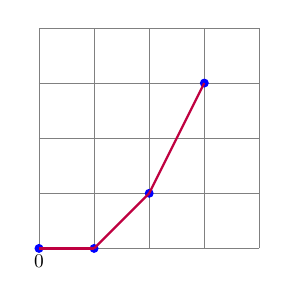
\begin{tikzpicture}[scale=0.7, transform shape]
    \draw[gray, very thin] (0,0) grid (4,4); 

    \node[below] at (0,0) {0};
    \filldraw[blue] (0,0) circle (2pt);
    \filldraw[blue] (1,0) circle (2pt);
    \filldraw[blue] (2,1) circle (2pt);
    \filldraw[blue] (3,3) circle (2pt);

    \draw[thick, purple] (0,0) -- (1,0);
    \draw[thick, purple] (1,0) -- (2,1);
    \draw[thick, purple] (2,1) -- (3,3);
\end{tikzpicture}
\end{center}

Observe the Newton ploygon has $3$ distinct slopes $0, 1, 2$, $f(x)$ splits
over $\Q_2$.  If $f(x)$ is irreducible over $\Q$, then $E :=
\Q[x]/(f(x))$ is a degree $3$ extension where the prime $(2) \normal \Z$
splits.

\medbreak

Let $A$ be a DVR, $K = \Frac A$, a monic polynomial $f(x) = x^n + a_1x^{n-1} +
\cdots + a_{n-1}x + a_n \in K[x]$ is {\bf Eisenstein} \index{Eisenstein
    polynomial} if $\nu_A(a_i) \geq 1$, ($1 \leq i \leq n-1$) and $\nu_A(a_n) =
1$.  Equivalently, $f(x)$ is Eisenstein if and only if the Newton polygon
$N_K(f)$ has a single slope $1/n$ with multiplicity $n$.  We characterize
totally ramified and unramified extensions of CDVFs.

\begin{prop}~
    \label{prop:totally-ramified-cdvf}
    \begin{enumerate}
        \item Let $E/K$ be a totally ramified extension of CDVFs, let $f(x) \in
            K[x]$ be the minimal polynomial of a chosen uniformizer $\pi_E$ of
            $A_E$.  Then $f(x)$ is Eisenstein and $E = K(\pi_E)$.

        \item Let $K$ be a CDVF, $f(x) \in K[x]$ be a separable Eisenstein
            polynomial, $E := K[x]/(f(x))$.  Then $f(x)$ is irreducible over
            $K$, $E/K$ is totally ramified, and $x \bmod{f(x)} \in E$ is a
            uniformizer of $A_E$.
    \end{enumerate}
\end{prop}

\begin{proof}~
    \begin{enumerate}
        \item Let $L/E/K$ be the Galois closure of $E/K$, and $f(x)$ factorizes as
            $f(x) = (x - \pi_E) (x - \alpha_2) \cdots (x - \alpha_n)$ over $L$.
            Since $\nu_L(\cdot)$ is invariant under Galois action, $\nu_L(\pi_E)
            = \nu_L(\alpha_i) = e_{L/E}$ for all $i$.  So
            \begin{figure}[htpb]
            \begin{center}
            \begin{tikzpicture}[scale=0.8, transform shape]
                \node at (-1,0.75) {$N_L(f) = $};
                \draw[-Latex] (0,0) -- (3,0);
                \draw[-Latex] (0,0) -- (0,1.5);
                \draw[thick, purple] (0,0) -- (2.8,1.2);
                \filldraw[blue] (0,0) circle (2pt);
                \filldraw[blue] (2.8,1.2) circle (2pt);
                \node[right] at (2.8,1.2) {$(n, n \cdot e_{L/E})$};
            \end{tikzpicture}
            \quad
            \begin{tikzpicture}[scale=0.8, transform shape]
                \node at (-1,0.75) {$N_K(f) = $};
                \draw[-Latex] (0,0) -- (3,0);
                \draw[-Latex] (0,0) -- (0,1.5);
                \draw[thick, purple] (0,0) -- (2.8,0.6);
                \filldraw[blue] (0,0) circle (2pt);
                \filldraw[blue] (2.8,0.6) circle (2pt);
                \node[right] at (2.8,0.6) {$(n, n \cdot e_{L/E}/e_{L/K} = n/e_{E/K})$};
            \end{tikzpicture}
            \end{center}
            \end{figure}

            Since $\nu_K(a_n) \geq 1$ is an integer, we must have $n \geq
            e_{E/K}$.  On the other hand, since $E/K$ is totally ramified,
            $e_{E/K} = [E : K] \geq [K(\pi_E) : K] \geq n$, so $e_{E/K} = n$,
            $f(x) \in K[x]$ is Eisenstein and $K(\pi_E) = E$.

        \item Let $L$ be the splitting field of $f(x)$ over $K$, let $\alpha \in
            L$ be a root of $f(x)$.  We consider the tower $L/K(\alpha)/K$.
            Since $f(x)$ is Eisenstein over $K$,

            \begin{figure}[htpb]
            \begin{center}
            \begin{tikzpicture}[scale=0.65, transform shape]
                \node at (-1,0.75) {$N_K(f) = $};
                \draw[-Latex] (0,0) -- (3,0);
                \draw[-Latex] (0,0) -- (0,1.5);
                \draw[thick, purple] (0,0) -- (2.8,0.8);
                \filldraw[blue] (0,0) circle (2pt);
                \filldraw[blue] (2.8,0.8) circle (2pt);
                \node[right] at (2.8,0.8) {$(n, 1)$};
            \end{tikzpicture}
            \quad
            \begin{tikzpicture}[scale=0.65, transform shape]
                \node at (-1.2,0.75) {$N_{K(\alpha)}(f) = $};
                \draw[-Latex] (0,0) -- (3,0);
                \draw[-Latex] (0,0) -- (0,1.5);
                \draw[thick, purple] (0,0) -- (2.8,1.2);
                \filldraw[blue] (0,0) circle (2pt);
                \filldraw[blue] (2.8,1.2) circle (2pt);
                \node[right] at (2.8,1.2) {$(n, e_{K(\alpha)/K})$};
            \end{tikzpicture}
            \quad
            \begin{tikzpicture}[scale=0.65, transform shape]
                \node at (-1,0.75) {$N_{L}(f) = $};
                \draw[-Latex] (0,0) -- (3,0);
                \draw[-Latex] (0,0) -- (0,1.5);
                \draw[thick, purple] (0,0) -- (2.8,1.2);
                \filldraw[blue] (0,0) circle (2pt);
                \filldraw[blue] (2.8,1.2) circle (2pt);
                \node[right] at (2.8,1.2) {$(n, e_{L/K})$};
            \end{tikzpicture}
            \end{center}
            \end{figure}

            Since $N_L(f)$ has a single slope of $e_{L/K}/n = e_{L/K(\alpha)}
            \nu_{K(\alpha)}(\alpha)$, so $N_{K(\alpha)}(f)$ has a single slope
            of $e_{K(\alpha)/K}/n = \nu_{K(\alpha)}(\alpha)$, which is a
            positive integer.  In particular, $e_{K(\alpha)/K} \geq n$.  On the
            other hand, $e_{K(\alpha)/K} \leq [K(\alpha) : K] \leq n$, so
            $e_{K(\alpha)/K} = n$.  Hence $K[x]/(f(x)) \to K(\alpha)$, $\cls{x}
            \mapsto \alpha$ induces a surjective map between $K$-vector spaces,
            hence it is an isomorphism.  So $f(x)$ is irreducible and $E/K$ is a
            totally ramified extension of CDVFs and $\nu_E(x \bmod{f(x)}) =
            \nu_{K(\alpha)}(\alpha) = 1$, so $x \bmod{f(x)} \in E$ is a
            uniformizer of $A_E$.
    \end{enumerate}
\end{proof}

\begin{prop}
    \label{prop:unramified-cdvf}
    Let $K$ be a CDVF, $\ell/k_K$ a finite separable extension.  Then there
    exists an unramified extension $L/K$ of CDVFs and an isomorphism $i : \ell
    \to k_L$ satisfying the following universal property:  for any extension
    $E/K$ of CDVFs and $k_K$-embeddings $j : \ell \hookrightarrow k_E$, there is a
    unique $K$-embedding $J : L \to E$ such that the following diagram commutes:
    \[
      \begin{tikzcd}
        & k_L \ar{rd}{J|_{A_L} \bmod{\pi_L}} &\\
        \ell \ar{ru}{i}[swap]{\sim} \ar[hook]{rr}{j} & & k_E
      \end{tikzcd}
    \]
\end{prop}


\begin{proof}
    Let $\cls{\alpha} \in \ell$ be a primitive element, let $\cls{f}(x) \in
    k_K[x]$ be the minimal polynomial of $\cls{\alpha}$, let $f(x) \in A_K[x]$
    be a monic lift of $\cls{f}(x)$, define $L := K[x]/(f(x))$, let $\alpha$
    denote the residue class $x \bmod{f(x)}$.
    Since $\cls{f}(x)$ is irreducible and separable, so is $f(x)$, so $L/K$ is a
    separable extension of CDVFs.  There is an inclusion $A_K[x] \hookrightarrow
    L[x]$, note the image lands in $A_L[x]$ and $f(x)$ is mapped to zero, so we
    have map $A_K[x]/(f(x)) \to A_L[x]$.  Since $(\pi_K) \subseteq
    (\pi_L)$, this induces map $i : \ell = k_K[x]/(\cls{f}(x)) = A_K[x]/(\pi_K,
    f(x)) \to A_L[x]/(\pi_L) = k_L$ of $k_K$-algebras.  Since this map is
    nonzero, it must be an $k_K$-embedding.  Since $f_{L/K} = [k_L : k_K] \leq
    [L : K] = \deg f(x) = \deg \cls{f}(x) = [\ell : k_K]$, the map $i : \ell \to
    k_L$ must be an isomorphism.

    Let $E/K$ be another extension of CDVFs with a $k_K$-embedding $j : \ell
    \hookrightarrow k_E$.  Such embedding is determined by a root $\cls{\theta}$
    of $\cls{f}(x)$ in $k_E$.  Since $\cls{f}(x)$ is separable, such root is
    simple, and by Hensel's Lemma, $\exists!\ \theta \in A_E$ such that
    $f(\theta) = 0$ and $\theta \bmod{\pi_E} = \cls{\theta}$.  So any such
    embedding is determined by a root of $f(x)$ in $E$, hence determines a
    unique embedding $J : L \to E$ such that $\cls{J} \circ i = j : \ell \to
    k_E$.
\end{proof}

In particular, since any finite field $\F_p$ has a unique degree $n$ separable
extension $\F_{p^n}/\F_p$ for all $n \in \Z_{\geq 1}$, the $p$-adic field $\Q_p$
has a unique unramified extension $E_{p^n}$ together with an isomorphism
$\F_{p^n} \oto{\sim} k_{E^{p^n}}$.


As another consequence of the characterization, for any extension $E/K$ of CDVFs
with $k_E/k_K$ separable, there is an unramified extension $E_0/K$ with $k_E
\iso k_{E_0}$ and a $K$-embedding $E_0 \hookrightarrow E$.  Identify $E_0$ with
its image in $E$, we get a tower $E/E_0/K$.  For any unramified subextension
$E/L/K$, we have a $k_K$-embedding $k_L \hookrightarrow k_E = k_{E_0}$, hence
the embedding lifts to a $K$-embedding $L \hookrightarrow E_0$.  Hence $E_0/K$
is the {\bf maximal unramified subextension} of $E/K$ \index{maximal unramified
    subextension}.

Intuitively, the maximal unramified subextension should be the subfield with
``no inertia'', i.e., it should be the fixed field of the inertia group.  This is
indeed the case.

\begin{prop}
    Let $E/K$ be a Galois extension of CDVFs with $k_E/k_K$ separable, then $E_0
    \iso E^{I_{E/K}}$, where $I_{E/K} = \SetForm{\sigma \in
        \Gal(E/K)}{\sigma|_{A_E} \bmod{\pi_E} = \id_{k_E}}$ is the inertia
    subgroup.
\end{prop}

\begin{proof}
    We adopt the construction in \Cref{prop:unramified-cdvf}.  Since $E/K$ is
    Galois and $k_E/k_K$ is separable, $k_E/k_K$ is Galois, so $k_E$ contains
    all roots of $\cls{f}(x)$.  Since $\cls{f}(x)$ is separable, by Hensel's
    Lemma, $E$ contains all roots of $f(x)$, so $E_0/K$ is Galois.  By
    Galois theory, it suffices to show $\Gal(E/E_0) = I_{E/K}$.  Since Hensel's
    Lemma gives us a bijection between roots of $\cls{f}(x)$ in $k_E$ and roots
    of $f(x)$ in $E$, for $\sigma \in \Gal(E/K)$, $\sigma \in I_{E/K}$ iff
    $\cls{\sigma} \in \Gal(k_E/k_K)$ fixes all roots of $\cls{f}(x)$ iff
    $\sigma$ fixes $E_0$.
\end{proof}

This suggests us a way to investigate the question of ``how ramified an
extension of CDVFs is''.  If $E/K$ is an Galois extension of CDVFs with
$k_E/k_K$ separable, then we have tower $E/E_0 = E^{I_{E/K}}/K$, where $E_0/K$
is unramified and $E/E_0$ is totally ramified.  Then we hope to investigate how
ramified $E/E_0$ is by looking at various subgroups of the inertia group.  We
introduce the notion of ramification groups to do just that.

\medbreak

\marginnote{Setup:\\ $E/K$ Galois extension of CDVFs, $k_E/k_K$ separable}[0cm]

Unless otherwise mentioned, all extensions $E/K$ below will be Galois and
$k_E/k_K$ separable, let $G := \Gal(E/K)$ denote the Galois group, let $\pi_E,
\pi_K$ be some uniformizers of $A_E, A_K$ respectively.  We first observe $A_E$
could be generated by a single element $\alpha$, $A_E = A_K[\alpha]$.

\begin{proof}
    Suppose $k_E = k_K(\cls{y})$, let $\cls{p}(x) \in k_K[x]$ be the minimal
    polynomial of $\cls{y}$, $p(x) \in A_K[x]$ a monic lift of $\cls{f}(x)$.
    Since $\cls{p}(x)$ is separable, by Hensel's Lemma, $\exists!\ y \in A_E$
    such that $p(y) = 0$ and $y \bmod{\pi_E} = \cls{y}$.  Consider the element
    $\alpha := y + \pi_E \in A_E$.  Observe by Taylor expansion, $p(y + \pi_E) =
    \pi_E p'(y) + \pi_E^2 z$.  Since $\cls{p'}(y) \neq 0$, we have $\nu_E(p(y +
    \pi_E)) = 1$, so $p(y + \pi_E)$ is an uniformizer of $A_E$.  Also observe
    the map $A_K[y + \pi_E] \to k_E$ sending $y + \pi_E$ to $\cls{y}$ is
    surjective.  Hence every element of $A_E$ can be written as $\sum_{i \geq 0}
    a_i p(y + \pi_E)^i$, where $a_i \in X$, and $X \subseteq A_K[y + \pi_E]$ a
    set of representatives of residue classes in $k_E$.

    Since $A_E$ is finite as a $A_K$ module, and by the observation above
    $A_E/(\pi_K) = A_E/(\pi_E^{e_{E/K}})$ is generated by $y + \pi_E$, it
    follows by NAK that $A_E = A_K[y + \pi_E]$.
\end{proof}

\marginnote{Remark:\\ the function $i_G$ may be defined using any uniformizer
    $\pi_E$, we choose $\alpha$ for simplicity}[0cm]

Define function $i_G : G \to \Z$, $i_G(\sigma) := \nu_E(\sigma(\alpha) -
\alpha)$ \index{$i_G(\cdot)$}.   And define the {\bf $i$-th lower ramification
    group} \index{ramification group (lower index)} $G_i$ to be
\begin{align*}
    G_i
    & := \SetForm{\sigma \in G}{i_G(\sigma) \geq i + 1}\\
    & = \SetForm{\sigma \in G}{\nu_E(\sigma(\alpha) - \alpha) \geq i + 1}\\
    & = \SetForm{\sigma \in G}{\sigma|_{A_E} \bmod{\pi_E^{i+1}} = \id \in
        \Aut(A_E/(\pi_E^{i+1}))}.
\end{align*}

If $\sigma \in G_i$, $\tau \in G$, then $\cls{\tau \sigma \tau^{-1}} =
\cls{\tau} \cls{\sigma} \cls{\tau}^{-1} = \cls{\tau}\cls{\tau}^{-1} = \id \in
\Aut(A_E/(\pi_E^{i+1}))$.  So $G_i \normal G$ for all $i \geq -1$.  Note by
definition $\cap_{i \geq -1} G_i = 1$, so we get a filtration of $G$
\[
    G = G_{-1} \geq G_0 = I_{E/K} \geq G_1 \geq G_2 \geq \cdots \geq G_N = 1.
\]

\begin{remark}
    For $\sigma, \tau \in G$, one has $i_G(\sigma \tau) \geq \min\{i_G(\sigma),
    i_G(\tau)\}$, with equality if and only if $i_G(\sigma) \neq i_G(\tau)$.

    Why? suppose $i_G(\sigma) = a$ and $i_G(\tau) = b$, then $\sigma(\pi_E) =
    \pi_E + \pi_E^a u_1$ and $\tau(\pi_E) = \pi_E + \pi_E^b u_2$, hence $\sigma
    \tau(\pi_E) = \pi_E + \pi_E^a z_1 + (\pi_E + \pi_E^a u_1)^b \sigma(u_2)$, so
    $i_{G}(\sigma \tau) = \min \{a, b \cdot \nu_E(\pi_E + \pi_E^a u_1)\}$.  If
    $a = 0$, it equals $0$; otherwise it equals $\min\{a, b\}$ as we wished.
\end{remark}

\begin{example}~
    \begin{enumerate}
        \item Consider the extension $\Q_2(\sqrt{2})/\Q_2$.  This is a totally
            ramified Galois extension of CDVFs since the minimal polynomial of
            $\sqrt{2}$ is Eisenstein. We have $G = \{1, \tau\} = I_{E/K} = G_{0}
            = G_{-1}$, where $\tau : \sqrt{2} \mapsto -\sqrt{2}$.  Since
            $\sqrt{2}$ is a uniformizer, and $i_G(\tau) = \nu_E(-2\sqrt{2}) =
            3$, we have $G_{-1} = G_{0} = G_1 = G_2 = \{1, \tau\}$ and $G_3 =
            \{1\}$.

        \item Consider the extension $\Q_2(i)/\Q_2$, the minimal polynomial of
            $i + 1$ is $(x-1)^2 + 1 = x^2 - 2x + 2$, which is Eisenstein, so
            this is a totally ramified Galois extension of CDVFs with
            uniformizer $i + 1$.  We have $G = \{1, \tau\} = I_{E/K} = G_{0} =
            G_{-1}$, where $\tau : i \mapsto -i$.  Since $i_G(\tau) = \nu_E(-2i)
            = \nu_E((1 + i)^2) = 2$, we have $G_{-1} = G_0 = G_1 = \{1, \tau\}$
            and $G_2 = \{1\}$.
    \end{enumerate}
    Intuitively, $\Q_2(\sqrt{2})/\Q_2$ is more ramified than $\Q_2(i)/\Q_2$.
\end{example}

\medbreak

Observe by definition, if $H \leq G$ is a subgroup, $K' := E^H$, identify $H$
with $\Gal(G/K')$, then $H_i = G_i \cap H$.  However it is not generally true
that given $H \normal G$, we have $(G/H)_i = G_iH/H$.  In the rest of the
section we will

\begin{enumerate}
    \item[(1)] Investigate the structure of the filtration $G = G_{-1} \geq G_0
        \geq G_1 \geq G_2 \geq \cdots$.
    \item[(2)] Fix the problem that ramification groups are incompatible with
        quotients.
\end{enumerate}

\subsection{Structure of the filtration by lower ramification groups}

Define {\bf unit groups} \index{unit groups $U_E^{{(i)}}$} $U_E^{(0)} = U_E :=
A_E^{\times}$ and $U_E^{(i)} := \Ker(A_E^{\times} \to
(A_E/(\pi_E)^i)^{\times})$.  So we get a filtration of unit groups $U_E^{(0)}
\geq U_E^{(1)} \geq U_E^{(2)} \geq \cdots$.  Observe we have group isomorphisms
$U_E^{(i)}/U_E^{(i+1)} \to \pi_E^i A_E / \pi_E^{i+1} A_E$ induced by the map
$\alpha \in U_E^{(i)} \mapsto \alpha - 1 \in \pi_E^{i} A_E$.  Why is this a
group map?  Let $\alpha, \beta \in U_E^{(i)}$, we want to show $(\alpha\beta -
1) - (\alpha - 1) - (\beta - 1) \in \pi_E^{i+1} A_E$.  Note it equals $\alpha
(\beta - 1) - (\beta - 1) = (\alpha - 1) (\beta - 1)$.  Since $\alpha - 1, \beta
- 1 \in \pi_E^i$, their product is divisible by $\pi_E^{i+1}$.

\medbreak

Why do we care about unit groups?  Because we have the following equivalence:
for $\sigma \in G$,
\begin{align*}
    \sigma \in G_i
    & \iff i_G(\sigma) \geq i+1 \iff 
    \nu_E(\sigma(\pi_E) - \pi_E) \geq i+1\\
    & \iff \nu_E\del{\frac{\sigma(\pi_E)}{\pi_E} - 1} \geq i
    \iff \frac{\sigma(\pi_E)}{\pi_E} \in 1 + \pi_E^i A_E = U_E^{(i)}.
\end{align*}
So we get an injective group maps $G_i/G_{i+1} \hookrightarrow
U_E^{(i)}/U_E^{(i+1)}$.  In particular, we have
\[
    G_0/G_1 \hookrightarrow U_E^{(0)}/U_E^{(1)} \iso k_E^{\times}, \qquad
    G_i/G_{i+1} \hookrightarrow \pi^i A_E / \pi^{i+1} A_E \quad (i \geq 1).
\]
So $G_0/G_1$ is cyclic and $G_i/G_{i+1}$ are abelian $(i \geq 1)$.  In
particular $G_0$ is solvable.  So if the quotient $G/G_0 = G/I_{E/K} \iso
\Gal(k_E/k_K)$ is solvable, then the whole Galois group $G = \Gal(E/K)$ is
solvable.   Recall finite extensions of a finite field are cyclic, so if $k_K$
is a finite field, then for any $E/K$ Galois CDVF extension, $k_E/k_K$
separable, $E/K$ is solvable.  In particular, there are no Galois extension of
CDVFs $E/K$, $k_E/k_K$ separable, $k_K$ finite, with $\Gal(E/K) \iso A_5$.

\medbreak

We have a finer description of the quotients.  Suppose $\ch k_E = 0$, then each
quotient $\pi_E^{i} / \pi_E^{i+1}$ is a $\Q$-vector space, and hence each
quotient $G_i/G_{i+1}$ is a finite subgroup of a $\Q$-vector space, hence must
be trivial.  Since for $i \gg 0$, $G_i = 0$, all of $G_i$ $(i \geq 1)$ must be
trivial.  So $G_0 \leq k_E^{\times}$ is finite cyclic.

Suppose $\ch k_E = p > 0$, then each $\pi_E^{i} / \pi_E^{i+1}$ $(i \geq 1)$ is a
finite dimensional $\F_p$-vector space, so have order some $p$ power.  So $G_1$
is a $p$-subgroup of $G_0$.  Furthermore, since $G_0/G_1 \leq k_E^{\times}$ is
cyclic of order coprime to $p$,  $G_1 \normal G_0$ is a $p$-Sylow subgroup.

\begin{defn}[tame/wild ramification]
    Let $E/K$ be a Galois extension of CDVFs with $k_E/k_K$ separable.  We say
    $E/K$ is {\bf tamely ramified} \index{tame ramification} if $G_1 = 1$,
    otherwise we say it is {\bf wildly ramified} \index{wild ramification}.
\end{defn}

\begin{remark}
    $E/K$ is tamely ramified if and only if $\ch k_E = 0$, or $\ch k_E = p > 0$
    and $p \nmid \abs{G_0} = e_{E/K}$.
\end{remark}

\begin{remark}
    If $E/K$ is tamely and totally ramified, $\abs{G} = \abs{G_0} = e_{E/K} = [E
    : K]$ divides $\abs{k_E^{\times}}$.  So we could get some information of the
    size of the Galois group using information of the size of $k_E^{\times}$.
\end{remark}

\medskip

We give a characterization of tamely and totally ramified extensions $E/K$.

\begin{prop}
    Let $E/K$ be tamely and totally ramified, then there exists uniformizer
    $\pi_K$ of $A_K$ such that $A_E = A_K[\sqrt[n]{\pi_K}]$, where $n = [E :
    K]$.
\end{prop}

\begin{proof}
    Since $E/K$ is totally ramified, $e_{E/K} = n$, $G = G_0 = I_{E/K}$,
    $f_{E/K} = 1$, $k_E = k_K$.  Since $E/K$ is tamely ramified, $G = G_0
    \hookrightarrow k_K^\times$ , so $G \iso \Z/n$, so $k_K$ contains an element
    $\cls{\zeta}$ of order $n$.  Let $f(X) := X^n - 1$, note $f'(X) = nX^{n-1}$,
    so $\cls{f}'(X) = n \cls{\zeta}^{n-1}$.  If $n = 0 \in k_K$, then $\ch k_K
    \mid n$, but this is absurd because finite subgroups of a field of
    characteristic $p$ are cyclic and of order coprime to $p$.  Hence
    $\cls{\zeta}$ is a primitive root of $\cls{f}(X)$, so by Hensel's lemma,
    there is a unique lift $\zeta \in A_K$ with $\zeta^n = 1$ and $\zeta \bmod
    \pi_K = \cls{\zeta}$.

    Let $\sigma \in G$ be a generator, consider the element
    \[
        \alpha := \pi_E  + \zeta^{-1} \sigma(\pi_E) + \zeta^{-2} \sigma^2(\pi_E)
        + \cdots + \zeta^{-(n-1)} \sigma^{n-1}(\pi_E) \in A_E.
    \]
    Note
    \[
        \sigma(\alpha) = \sigma(\pi_E) + \zeta^{-1} \sigma^2(\pi_E) + \cdots +
        \zeta^{-(n-2)} \sigma^{n-1}(\pi_E) + \zeta^{-(n-1)} \pi_E
        = \zeta \alpha.
    \]
    Hence $\sigma(\alpha^n) = \sigma(\alpha)^n = \zeta^n \alpha^n = \alpha^n$,
    so $\alpha^n$ is fixed by $G$, so $\alpha^n \in K \cap A_E = A_K$.
    Furthermore, since $\zeta \in A_K^\times \subseteq A_E^\times$,
    $\nu_E(\zeta) = 0$, and $\nu_E(\cdot)$ is preserved by $G$, so
    $\nu_E(\alpha) = \nu_E(n \pi_E) = \nu_E(\pi_E) = 1$, so $\alpha \in A_E$ is
    a uniformizer.  So $\nu_K(\alpha^n) = \nu_E(\alpha^n)/n = 1$, and $\alpha^n
    \in A_K$ is also a uniformizer.  Finally, since $k_K = k_E$, every element
    of $A_E$ may be expressed as $\sum_{i \geq 0} a_i \alpha^i$, where $a_i \in
    A_K$.  So $A_E = A_K[\alpha]$, we are done.
\end{proof}

\subsection{Fixing the indexing of the ramification groups}

We now fix the indexing of the ramification groups so that they are compatible
with quotients.  Recall the setup: $E/K$ a Galois extension of CDVFs with Galois
group $G$, $H \normal G$, $K' := E^H$.  We first observe some relations between
$i_G$ and $i_{G/H}$.

\begin{prop}
    \label{prop:tate-index}
    For every $\sigma \in G/H$,
    \[
        i_{G/H}(\sigma) = \frac{1}{e_{E/K'}} \sum_{s \in G : \cls{s} = \sigma
            \in G/H} i_G(s)
    \]
\end{prop}

\begin{proof}[Proof (Due to Tate)]
    Pick generators $x \in A_E$ and $y \in A_{K'}$ such that $A_E = A_K[x]$ and
    $A_{K'} = A_K[x]$.  Then for $sH \in G/H$, $i_{G/H}(sH) = \nu_{K'}(sH(y) -
    y) = \frac{1}{e_{E/K'}} \nu_E(s(y) - y)$.  Suffices to show for $s \in G$,
    \[
        \nu_E(s(y) - y) = \sum_{t \in H} \nu_E(st(x) - x)
        = \nu_E(\prod_{t \in H} (st(x) - x)),
    \]
    we may assume $s \not\in H$ because in that case both sides are infinite.

    \medskip

    \emph{Key observation:}  from Galois theory, we know the minimal polynomial
    of $x$ over $K'$ equals $f(X) = \prod_{t \in H} (t(x) - X)$.  This is
    because $H$ fixes the minimal polynomial, hence every $H$-conjugate of $x$
    is a root of the minimal polynomial.  For $s \in G$, let $s \cdot f(X)$
    denote the polynomial $f(X)$ with each coefficient acted upon by $s$.  So
    $\prod_{t \in H} (st(x) - x) = (s \cdot f)(x)$.

    \medskip

    Let $s \in G - H$ be fixed, let $a := s(y) - y$ and $b := \prod_{t \in H}
    (st(x) - x)$, we will show $(a) = (b) \normal A_E$.  Expand the minimal
    polynomial $f(X)$ into $\sum a_i X^i$, for $a_i \in A_E \cap K' = A_{K'}$.
    Since $A_{K'} = A_K[y]$, we have polynomials $f_i(X) \in A_K[X]$ such that
    $a_i = f_i(y)$.  Observe
    \[
        (s \cdot f)(X) - f(X)
        = \sum [s(a_i) - a_i] X^i
        = \sum [f_i(s(y) - y)] X^i.
    \]
    Since $\nu_E(f_i(s(y) - y)) \geq \nu_E(s(y) - y)$ (clear if $\deg f_i \geq
    1$, and if $\deg f_i = 0$, then $a_i \in A_K$, so $s(a_i) - a_i = 0$),
    $\nu_E((s \cdot f)(x)) = \nu_E((s \cdot f)(x) - f(x)) \geq \nu_E(s(y) - y)$,
    so $a \mid b$.

    Conversely, suppose $y = g(x)$ for $g(X) \in A_K[X]$, then $g(X) - y \in
    A_{K'}[X]$ has $x$ as a root, hence is divisible by $f(X)$, so $g(X) - y =
    f(X) \cdot h(X)$ in $A_{K'}[X]$.  Then $(s \cdot f)(X)$ divides $s \cdot
    g(X) - s(y) = g(X) - s(y)$, so $b = (s \cdot f)(x)$ divides $g(x) - s(y) =
    -a$. We win.
\end{proof}

\medskip

We make our first step toward the case of quotients.

\begin{prop}
    Suppose the normal subgroup $H \normal G$ equals some $G_j$ $(j \geq 0)$,
    then $(G/H)_i = G_i/H$ for $(i \leq j)$ and $(G/H)_i = 1$ for $i \geq j$.
\end{prop}

\begin{proof}
    Note $G/H = G_{-1}/H \geq G_0/H \geq G_1/H \cdots \geq G_j/H = 1$ is a
    filtration of $G/H$, so for any $\sigma \neq \id \in G/H$, there is some $i
    \geq -1$ such that $\sigma \in G_i/H$ but $\sigma \not\in G_{i+1}/H$.  So
    any representative $s \in G$ of $\sigma$ is contained in $G_i - G_{i+1}$, so
    $i_G(s) = i+1$.  So \Cref{prop:tate-index} tells us $i_{G/H}(\sigma) =
    \abs{H} (i+1) / e_{E/K'}$.

    Furthermore, since $H \leq G_0$, the fixed field $K' = E^H$ is an
    intermediate field between $E$ and $E_0 = E^{G_0}$, in particular $E/K'$ is
    totally ramified, and $e_{E/K'} = [E : K'] = \abs{H}$.  So $i_{G/H}(\sigma)
    = i+1$.  So $G_i/H = (G/H)_i$ for $-1 \leq i \leq j$.  And for $i \geq j$,
    $(G/H)_i \leq (G/H)_j = G_j/G_j = 1$, they are all trivial.
\end{proof}

We want to modify the indexing so that the above is true for any normal subgroup
$H \normal G$.  We introduce the upper ramification indexing as following.

For any real number $u \geq 0$, let $G_u := G_{\ceil{u}}$.  Define {\bf
    ramification function} \index{ramification function} $\varphi_{E/K} : [0,
\infty) \to [0, \infty)$ by
\[
    \varphi_{E/K}(u) := \int_{0}^{u} [G_0 : G_t]^{-1} dt.
\]
Note $\varphi_{E/K}$ is continuous, piecewise linear, strictly increasing, and
the discontinuities of its derivative occurs only at the integer values of $u$.
Let $\psi_{E/K}$ denote its inverse: $\psi_{E/K}(v) := \varphi_{E/K}^{-1}(v)$
for $v \in [0, \infty)$.  So $\psi_{E/K}$ is also a strictly increasing
piecewise linear function from $[0, \infty)$ to $[0, \infty)$, with slopes of
each linear segment the reciprocals of the slopes of segments of
$\varphi_{E/K}$. Define the {\bf upper ramification groups} \index{upper
    ramification groups} to be $G^{v} := G_{\psi_{E/K}(v)}$.

This definition is precisely the one we need to have $(G/H)^v = G^v H/H$ for all
$v$.  To see that, we need several numerical identities.

\begin{lem}
    \label{lem:phi_EK}
    \[
        \varphi_{E/K}(u) + 1 = \frac{1}{\abs{G_0}} \sum_{s \in G} \min \{i_G(s),
        u + 1\}.
    \]
\end{lem}

\begin{proof}
    Observe both sides are piecewise linear and equals $1$ at $0$.  So it
    suffices to check their derivatives are the same on each linear piece $[m,
    m+1]$.  Note if $m \leq u \leq m +1$, then the derivative of LHS is $[G_0 :
    G_u]^{-1}$ and the derivative of RHS is
    \[
        \frac{1}{\abs{G_0}} \sum_{s \in G : i_G(s) \geq u+1} 1
        = \frac{1}{\abs{G_0}} \sum_{s \in G_u} 1
        = [G_0 : G_u]^{-1},
    \]
    because $i_G(s) \geq u+1 \iff s \in G_u$.  We win.
\end{proof}

\begin{lem}
    \label{lem:i_G/H_phi_E/K'}
    For $\sigma \in G/H$, let $j(\sigma)$ denote the least upper bound of
    $i_G(s)$ as $s$ runs through all representatives of $\sigma$ in $G$. Then
    \[
        i_{G/H}(\sigma) - 1 = \varphi_{E/K'}(j(\sigma) - 1).
    \]
\end{lem}

\begin{proof}
    Pick representative $s$ of $\sigma$ so that $i_G(s) \geq i_G(st)$ for all $t
    \in H$, hence $j(\sigma) = i_G(s)$.  Expand both sides using
    \Cref{lem:phi_EK} and \Cref{prop:tate-index}, we want to show
    \[
        \frac{1}{e_{E/K'}} \sum_{t \in H} i_G(st)
        = \frac{1}{\abs{H_0}} \sum_{t \in H} \min \{ i_H(t), j(\sigma) \}.
    \]
    Recall $e_{E/K'} = \abs{I_{E/K'}} = \abs{H_0}$.  It suffices to show for
    each $t \in H$, $i_G(st) = \min\{i_H(t), j(\sigma)\}$.  Note $i_H(t) =
    \nu_E(t(\pi_E) - \pi_E) = i_G(t)$, so we want to show $i_G(st) = \min
    \{i_G(t), i_G(s)\}$.  Suppose $i_G(t) < i_G(s)$, then by an earlier remark,
    $LHS = i_G(t) = RHS$.  Suppose $i_G(t) \geq i_G(s)$, then $i_G(s) \leq
    i_G(st) \leq i_G(s)$, so $LHS = RHS = i_G(s)$.
\end{proof}

\begin{thm}[Herbrand's Theorem]
    \label{thm:herbrand}
    If $v = \varphi_{E/K'}(u)$, then $G_u H / H = (G/H)_v$, where $G_u H / H$
    denotes the image of $G_u$ in the quotient $G/H$.
\end{thm}

\begin{proof}
    Let $\sigma = sH \in G/H$, then
    \begin{align*}
        \sigma \in G_u H / H
        & \iff \exists t \in H, st \in G_u &&\\
        & \iff \exists t \in H, i_G(st) \geq u + 1 &&\\
        & \iff j(\sigma) \geq u + 1 &&\\
        & \iff \varphi_{E/K'}(j(\sigma) - 1) \geq v && \varphi_{E/K'} \text{ is
        monotone}\\
        & \iff i_{G/H}(\sigma) \geq v + 1 && \text{\Cref{lem:i_G/H_phi_E/K'}}\\
        & \iff \sigma \in (G/H)_{v} &&.
    \end{align*}
\end{proof}

\begin{cor}
    The functions $\varphi, \psi$ satisfy the transitivity relations:
    \[
        \varphi_{E/K} = \varphi_{K'/K} \circ \varphi_{E/K'}, \quad
        \psi_{E/K} = \psi_{E/K'} \circ \psi_{K'/K}.
    \]
\end{cor}

\begin{proof}
    It suffices to show the case for $\varphi$, we will check the derivatives of
    both sides coincide on non-integer values.  Let $u \in (0, \infty)$ be a
    non-integer, $v := \varphi_{E/K'}(u)$, then
    \[
        (\varphi_{K'/K} \circ \varphi_{E/K'})'(u)
        = \varphi_{K'/K}'(v) \cdot \varphi_{E/K'}'(u)
        = [(G/H)_0 : (G/H)_v]^{-1} \cdot [H_0 : H_u]^{-1}
        = \frac{\abs{(G/H)_v} \abs{H_u}}{e_{K'/K} e_{E/K'}}.
    \]
    By \Cref{thm:herbrand}, the numerator equals $\abs{G_u H / H} \abs{H_u}$.
    Since we have short exact sequence
    \[
      \begin{tikzcd}
         0 \rar & H_u = G_u \cap H \rar & G_u \rar & G_u H / H \rar & 0
      \end{tikzcd}
    \]
    so the derivative equals $\abs{G_u}/e_{E/K} = [G_0 : G_u]^{-1} =
    \varphi_{E/K}'(u)$. We are done.
\end{proof}

\begin{cor}
    \[
        (G/H)^v = G^v H/H \qquad (v \geq 0).
    \]
\end{cor}

\begin{proof}
    \[
        (G/H)^v = (G/H)_{\psi_{K'/K}(v)}
        = G_{\psi_{E/K'} \circ \psi_{K'/K}(v)} H / H
        = G_{\psi_{E/K}(v)} H / H
        = G^v H / H.
    \]
\end{proof}


\subsection{Generalization and applications}

We are now able to generalize the notion of ``maximal unramified subextension''
to non Galois extensions of CDVFs with separable residue extensions.

\begin{defn}
    Let $E/K$ be any extension of CDVFs with $k_E/k_K$ separable, let $v \geq 0$
    be a real number.   Define subextension $K \subseteq E^v \subseteq E$ to be
    $E^v := E \cap L^{G^v}$, where $L/E$ is any extension of CDVFs, $k_L/k_E$
    separable, and $L/K$ Galois, and $G := \Gal(L/K)$.
\end{defn}

Some immediate observations:

\begin{enumerate}
    \item For $v < v'$, $\psi_{L/K}(v) < \psi_{L/K}(v')$, $G^v \geq G^{v'}$, so
        $E^v \subseteq E^{v'}$.
    \item Since $G^v = 1$ for $v \gg 0$ (recall $\psi_{E/K}$ is strictly
        increasing), so $\cup_{v \geq 0} E^v = E$.
    \item As $v$ increases from $0$, the field $E^v$ will start from the maximal
        unramified subextension of $E/K$ and become more and more ramified,
        until become the whole extension $E/K$.
    \item The definition of $E^v$ is independent of the choice of extension
        $L$.  Let $L, L'/E$ be two such extensions, the their compositum $L L'$
        in $\cls{E}$ is again an extension over $E$, Galois over $K$.  So it
        suffices to consider a tower $L' / L / E$, with $L'/K$ and $L/K$ Galois
        with Galois groups $G'$ and $G$, respectively.  Let $H := \Gal(L'/L)$.
        \[
          \begin{tikzcd}
            L' \dar[no head, swap]{H} \ar[no head, bend left]{dd}{G'}\\
            L \dar[no head, swap]{G}\\
            K
          \end{tikzcd}
        \]
        Recall from the compatibility of upper indexing with quotients, $G^v =
        (G'/H)^v = G'^v H / H$, so $E \cap L^{G^v} = E \cap (L')^{G'^v}$.
\end{enumerate}

This definition allow us to study the ramification theory of CDVFs using
ramification groups, in the case that the extension is not Galois.  In
particular we have description of the maximal unramified subextension using
ramification groups.

\begin{prop}
    Let $E/K$ be a possibly non-Galois extension of CDVFs with $k_E/k_K$
    separable, then
    \begin{enumerate}
        \item $E^0$ is the maximal unramified subextension of $E/K$.
        \item If $E/M/K$ is an intermediate field, then $M^v = E^v \cap M$.
        \item Let $E/M, N/K$ be two intermediate fields, then $M^v \cdot N^v
            \subseteq (M \cdot N)^v$.  In particular, if $M^v = M$ and $N^v =
            N$, then $M^v \cdot N^v = (M \cdot N)^v$.
    \end{enumerate}
\end{prop}

\begin{proof}
    Let $L/K$ be the Galois closure of $E/K$ (we know exists because any
    extension of CDVFs is assumed to be separable), let $G = \Gal(L/K)$, then
    $G^0 = G_0 = I_{L/K}$, and $L^{I_{L/K}} = L_0$ is the maximal unramified
    subextension of $L/K$.  So $E_0 \subseteq L_0 \cap E = E^0$.  On the other hand by
    the multiplicative property of residue degrees in towers, $E^0 = L_0 \cap E$
    is unramified over $K$, so $E^0 = E_0$ is the maximal unramified
    subextension of $E/K$.

    Part (2) follows from definition of $E^v$ and $M^v$.  For part (3), $M^v
    \cdot N^v = (M \cap L^{G^v}) \cdot (N \cap L^{G^v}) = (M \cdot N) \cap
    L^{G^v} = (M \cdot N)^v$.
\end{proof}

\bigskip

Unlike the lower ramification filtration, the upper ramification filtration
could jump on rational values.  However for most examples we care about, the
jumps can only be integers: this is the Hasse-Arf theorem.  It is stated below,
we will not prove it.

\begin{thm}[Hasse-Arf]
    Let $K/\Q_p$ be a finite extension, $E/K$ an abelian extension, then any
    jump of the upper ramification filtration of $\Gal(E/K)$ is an integer.
\end{thm}

To conclude this section we introduce an important notion that will be used to
organize the global class field theory -- the conductor ideal.  Let $K/\Q_p$ be
a finite extension, $E/K$ an abelian extension, the {\bf conductor ideal}
\index{(local) conductor ideal} $C_{E/K} \normal A_K$ is $(\pi_K^a)$, where $a$
is the smallest non-negative integer such that $\Gal(E/K)^a = 1$, or
equivalently $E^a = E$.

\begin{remark}
    $E/K$ unramified iff $E^0 = E$ iff $C_{E/K} = (\pi_K^0) = (1)$.
\end{remark}

\begin{prop}
    Let $K/\Q_p$ be a finite extension, $E/K$ an abelian extension, $E/E_1,
    E_2/K$ two abelian subextensions.  Then $E_1 \cdot E_2/K$ is also abelian,
    and $C_{E_1 \cdot E_2 / K} = \lcm(C_{E_1/K}, C_{E_2/K})$.
\end{prop}

\begin{proof}
    Observe we have inclusion of Galois groups $\Gal(E_1 \cdot E_2/K)
    \hookrightarrow \Gal(E_1/K) \times \Gal(E_2/K)$, so $E_1 \cdot E_2/K$ is
    abelian.  We also have in this case, $(E_1 \cdot E_2)^v = E_1 \cdot E_2$ if
    and only if $(E_1)^v = E_1$ and $(E_2)^v = E_2$.  Why? We know one direction
    from previous discussions.  Conversely note since $E_1 \cdot E_2/K$ is
    abelian, so $(E_i)^v = E_i \cap (E_1 \cdot E_2)^v = E_i \cap E_1 \cdot E_2 =
    E_i$.
\end{proof}

\section{Global Class Field Theory}

The goal of this section is to classify all abelian extensions of a fixed number
field $K$.  We will not prove the main theorem of global class field theory.
Instead we will understand the statement and its implications.

\medbreak

Let $E/K$ be an abelian extension of number fields. We start our discussion by
defining a global {\bf conductor ideal} \index{(global) conductor ideal}
$C_{E/K} \normal \cO_K$.  Define $C_{E/K} := \prod_{0 \neq \fp \in \Spec \cO_K}
\fp^{a_\fp}$, where $a_\fp$ is the smallest non-negative integer such that for
any $\fq \in \Spec \cO_E$ lying above $\fp$, $E_\fq^{a_\fp} = E_\fq$.  Since
$E/K$ is Galois, the Galois group acts transitively on the set of primes of
$\cO_E$ lying above $\fp$, so there is an isomorphism of extensions CDVFs
$E_{\fq_1} \oto{\sim} E_{\fq_2}$ over $K_{\fp}$ for $\fq_1, \fq_2$ lying above
$\fp$.  So the exponent $a_{\fp}$ equals the smallest non-negative integer such
that $E_{\fq_i}^{a_\fp} = E_{\fq_i}$ for each $\fq_i$ lying above $\fp$.
Therefore $C_{E/K} \cdot \cO_{K, \fp} = C_{E_{\fq}/K_{\fp}}$ for any $\fq$ lying
above $\fp$, where the right hand side is the local conductor ideal we have
introduced earlier.

We also note a prime $\fp \in \Spec \cO_K$ is ramified in $E$ if and only if
$\fp \mid C_{E/K}$.  So the conductor ideal describes those primes of $\cO_K$
that could ramify in $E$.  To see the use of this notion, we consider the
special case of classifying abelian extensions of $K = \Q$.

\medskip

First recall if $\zeta_N$ denotes a primitive $N$-th root of unity, then
$\Q(\zeta_N)/\Q$ is an abelian extension with Galois group isomorphic to
$(\Z\slash N)^{\times}$.  The isomorphism is given by sending $\sigma \in
\Gal(\Q(\zeta_N)/\Q) \mapsto a \in (\Z\slash N)^{\times}$ so that $\sigma(\zeta_N) =
\zeta_N^a$.  Hence by Galois theory, we have bijection
\[
  \begin{tikzcd}
      \left\{
          \parbox{6em}
          {subextensions $ \Q(\zeta_N) / K / \Q$}
      \right\}
      \rar[leftrightarrow]
      &
      \left\{
          \parbox{6em}
          {subgroups $ H \leq (\Z\slash N)^{\times} $}
      \right\}.
  \end{tikzcd}
\]

We also have

\begin{thm}[Kronecker-Weber]
    Let $K/\Q$ be an abelian extension, then there exists an integer $N \geq 1$
    such that $K \subseteq \Q(\zeta_N)$.  More precisely, $K \subseteq
    \Q(\zeta_N)$ if and only if $C_{K/\Q} \mid (N)$.  So for integer $N \geq 1$,
    we have a bijection
    \[
      \begin{tikzcd}
          \left\{
              \parbox{11em}
              {abelian extensions $K / \Q $ with $C_{K/\Q} \mid (N)$}
          \right\}
          \rar[leftrightarrow]
          &
          \left\{
              \parbox{6em}
              {subgroups $H \leq (\Z\slash N)^{\times}$}
          \right\}
      \end{tikzcd}
    \]
\end{thm}

We formulate the class field theory for cyclotomic fields.

\begin{thm}[Class field theory for cyclotomic fields]
    \label{thm:cft-cyclotomic}
    Let $N \geq 1$ be an integer, $K/\Q$ an abelian extension such that
    $C_{K/\Q} \mid N$.  So for any prime $p$ not dividing  $N$ must be
    unramified in $K$, so the Artin symbol $\genfrac(){}{}{K/\Q}{(p)}
    \in \Gal(K/\Q)$ is well-defined.  Then there exists a unique surjective
    group homomorphism $\phi_{K/\Q} : (\Z\slash N)^{\times} \epi \Gal(K/\Q)$
    that sends any residue class of prime $p \nmid N$ to the Actin symbol
    $\genfrac(){}{}{K/\Q}{(p)}$.    Furthermore, the map $K \mapsto \ker
    (\phi_{K/\Q})$ defines the bijection above
    \[
      \begin{tikzcd}[row sep=0ex]
          \left\{
              \parbox{11em}
              {abelian extensions $K / \Q $ with $C_{K/\Q} \mid (N)$}
          \right\}
          \rar[leftrightarrow]
          &
          \left\{
              \parbox{6em}
              {subgroups $H \leq (\Z\slash N)^{\times}$}
          \right\}\\
          K \rar[mapsto] & \ker(\phi_{K/\Q})
      \end{tikzcd}
    \]
\end{thm}

\bigskip

To generalize all of this to the case of an arbitrary number field $K$, we
introduce the following notations.

\medskip

Let $K$ be a number field, a {\bf modulus} \index{modulus} is a pair $\fm =
(\fm_0, \fm_{\infty})$, where $\fm \normal \cO_K$ is an ideal and $\fm_{\infty}
\subseteq \Hom_{\Q}(K, \R)$ is some set of $\Q$-homomorphisms from $K$ into
$\R$.  The {\bf trivial modulus} \index{trivial modulus} is the pair $(\cO_K,
\varnothing)$.  For abelian extension $E/K$ of number fields, we have a
natural associated modulus $\fm_{E/K} := (C_{E/K}, \SetForm{\tau : K
    \hookrightarrow \R}{\not\exists\, \cls{\tau} : E \hookrightarrow \R,
    \cls{\tau}|_K = \tau})$.

\begin{defn}
    Let $K$ be a number field, $\fm = (\fm_0, \fm_{\infty})$ a modulus,
    \begin{align*}
        & \mathscr{I} := \{\text{nonzero fractional ideals of } \cO_K\}\\
        & \mathscr{P} := \{\text{nonzero principal fractional ideals of }
        \cO_K\}\\
        & H_K := \mathscr{I} / \mathscr{P} \quad \text{the usual ideal class
            group}\\
        & \mathscr{I}(\fm_0) := \{\text{nonzero fractional ideals of } \cO_K
        \text{ coprime to } \fm_0\}\\
        & \qquad \quad = \SetForm{I \in \mathscr{I}}{\forall\, 0 \neq \fp \in
            \Spec \cO_K, \nu_{\fp}(\fm_0) > 0 \implies \nu_{\fp}(I) = 0}\\
        & K(\fm_0) := \SetForm{\alpha \in K^{\times}}{\forall\, 0 \neq \fp \in
            \Spec \cO_K, \nu_{\fp}(\fm_0) > 0 \implies \nu_{\fp}(\alpha) = 0}\\
        & K_{\fm} := \SetForm{\alpha \in K^{\times}}{\parbox{25em}
            {$\forall\, 0 \neq \fp \in \Spec \cO_K, \nu_{\fp}(\fm_0) > 0
                \implies 1 \equiv \alpha \bmod{\fm_0 \cO_{K,\fp}}$\\
            $\forall\, \tau \in \fm_{\infty}, \tau(\alpha) > 0$}
        }\\
        & \mathscr{P}(\fm_0) := \SetForm{(\alpha)}{\alpha \in K(\fm_0)}\\
        & \mathscr{P}_\fm := \SetForm{(\alpha)}{\alpha \in K_{\fm}}\\
        & H(\fm) := \mathscr{I}(\fm_0) / \mathscr{P}_{\fm}
        \quad \text{the {\bf ray class group} of $(K, \fm)$ \index{ray class
                group}}
    \end{align*}
\end{defn}

Observe for the trivial modulus, the ray class group coincides the usual ideal
class group.  Moreover, the ray class group generalizes the notion of usual
ideal class group and the group $(\Z \slash N)^{\times}$ from the case of $K =
\Q$.

\begin{prop}
    \label{prop:compute-Hm}
    Let $K$ be a number field, $\fm = (\fm_0, \fm_{\infty})$ a modulus, then
    \begin{enumerate}
        \item the ray class group $H(\fm)$ is a finite abelian group,
        \item there are short exact sequences of abelian groups
            \[
              \begin{tikzcd}[row sep = 0ex]
                0 \rar & \mathscr{P}(\fm_0) / \mathscr{P}_{\fm} \rar
                & H(\fm) = \mathscr{I}(\fm_0) / \mathscr{P}_{\fm} \rar
                & H_K \rar & 0\\
                0 \rar & \frac{\cO_K^\times}{\cO_K^\times \cap K_\fm} \rar
                & (\cO_K / \fm_0)^{\times} \times \prod_{\tau \in \fm_{\infty}}
                \{\pm 1\}  \rar& \frac{ \mathscr{P}(\fm) }{ \mathscr{P}_{\fm} }
                \rar& 0
              \end{tikzcd}
            \]
    \end{enumerate}
\end{prop}

\begin{proof}[Proof sketch.]
    Assume the result that the usual ideal class group $H_K$ is finite, the
    first part follows from the second.  To show the first sequence is short
    exact it suffices to show $H_K \iso \mathscr{I}(\fm_0) /
    \mathscr{P}(\fm_0)$.  Note we have injection $ \mathscr{I}(\fm) /
    \mathscr{P}(\fm_0) \hookrightarrow H_K $, to show surjectivity it suffices
    to show for each nonzero fractional ideal $I$ of $\cO_K$, there exists
    $\alpha \in K^\times$ so that $\alpha^{-1} I \in \mathscr{I}(\fm_0)$.  Put
    $\alpha := \prod_{\fp : \nu_{\fp}(\fm_0) > 0} \pi_\fp^{\nu_{\fp}(I)}$
    suffices.

    For the second sequence, note we have commutative diagram with exact rows:
    \[
      \begin{tikzcd}
         0 \rar & \cO_K^\times \cap K_\fm \rar \dar[hook] & K_\fm \rar
         \dar[hook] & \mathscr{P}_{\fm} \dar[hook] \rar & 0\\
         0 \rar & \cO_K^{\times} \rar & K(\fm_0) \rar & \mathscr{P}(\fm_0) \rar
         & 0
      \end{tikzcd}
    \]
    so by snakes lemma, we have short exact sequence
    \[
      \begin{tikzcd}
         0 \rar & \frac{\cO_K^\times}{\cO_K^\times \cap K_\fm} \rar &
         \frac{K(\fm_0)}{K_\fm} \rar & \frac{ \mathscr{P}(\fm_0) }{
             \mathscr{P}_{\fm} } \rar & 0.
      \end{tikzcd}
    \]
    One can show the map
    \[
      \begin{tikzcd}[row sep = 0ex]
          \displaystyle
          \frac{K(\fm_0)}{K_\fm} \rar &
          \displaystyle
          (\cO_K / \fm_0)^{\times}
          \times \prod_{\tau \in \fm_{\infty}} \{\pm 1\} \rar &
          \displaystyle
          \prod_{\fp \text{ s.t.} \nu_{\fp}(\fm_0) > 0}
          \del{\cO_{K, \fp}^{\times} \slash 1 + \fm_0 \cO_{K, \fp}}
          \times \prod_{\tau \in \fm_{\infty}} \R \slash \R_{> 0}\\
          \alpha \ar[mapsto]{rr} & & ((\alpha)_{\fp}, \tau(\alpha))
      \end{tikzcd}
    \]
    is an isomorphism.  Some observations/hints:

    \begin{enumerate}
        \item If $0 \neq \fp \in \Spec \cO_K$ such that $\nu_{\fp}(\fm_0) > 0$,
            then the inclusion $K^{\times} \hookrightarrow K_\fp^{\times}$
            restricts to $K(\fm_0) \hookrightarrow \cO_{K, \fp}^{\times}$,
            because the valuation at $\fp$ is zero.

        \item We have short exact sequence
            \[
              \begin{tikzcd}
                 0 \rar & 1 + \fm_0 \cO_{K, \fp} \rar & \cO_{K, \fp}^{\times}
                 \rar & (\cO_K / \fm_0)^{\times} \rar & 0
              \end{tikzcd}
            \]

        \item By Chinese remainder theorem, for any $x \in (\cO_K \slash
            \fm_0)^{\times}$, there exists $\alpha \in \cO_K$ with $\alpha
            \equiv x \bmod{\fm_0}$, replacing $\alpha$ with $\alpha + kN$ for
            some $k \in \N$ and $N \in \Z \cap \fm_0$, we may also assume
            $\tau(\alpha) > 0$.

        \item For any subset $S \subseteq \fm_{\infty}$, there exists $\alpha
            \in \cO_K$ such that $\alpha \equiv 1 \mod{\fp}$ for all $\fp$ with
            $\nu_{\fp}(\fm_0) > 0$, and $\tau(\alpha) = 1$ if $\tau \in S$ and
            $\tau(\alpha) = -1$ if $\tau \not\in S$.

        \item Let $\theta \in K$ be a primitive element, with minimal polynomial
            $f(X) \in \Q[X]$, then real embeddings of $K$ corresponds to real
            roots of $f(X)$.  Let $\alpha_\tau$ be the real root associated to
            $\tau \in S$, then fix a real polynomial $g(X) \in \R[X]$ such that
            $g(\alpha_\tau) = 1$ if $\tau \in S$ and $g(\alpha_\tau) = -1$ if
            $\tau \not\in S$.  Since $\Q$ is dense in $\R$, there exists $h(X)
            \in \Q[X]$ with $h(\alpha_\tau) > 0$ if $\tau \in S$ and
            $h(\alpha_\tau) < 0$ if $\tau \not\in S$.  Clear the denominators we
            may assume $h(X) \in \Z[X]$.  Let $\alpha \in \cO_K$ be any element
            such that $\alpha \equiv 1 \bmod{\fp}$ for $\nu_{\fp}(\fm_0) > 0$,
            and replace $\alpha$ by some $\alpha + kNh(\theta)$ for $k \gg 1$
            suffices.
    \end{enumerate}
\end{proof}

Here is the statement of global class field theory.

\begin{thm}[Global class field theory]
    Let $K$ be a number field, $\fm = (\fm_0, \fm_{\infty})$ a modulus of $K$.
    Then 
    \begin{enumerate}
        \item If $E/K$ is an abelian extension with $\fm_{E/K} \leq \fm$, then
            there exists a unique surjection $\phi_{E/K} : H(\fm) \epi
            \Gal(E/K)$ that sends each residue class $[\fp] \in H(\fm)$ to the
            Artin symbol $\genfrac(){}{}{E/K}{\fp}$.

        \item The map $E/K \mapsto \Ker(\phi_{E/K}) \leq H(\fm)$ defines an
            order-reversing bijection
            \[
              \begin{tikzcd}
                  \left\{
                      \parbox{11em}
                      {
                          abelian extensions $E/K$ with $\fm_{E/K} \leq \fm$
                      }
                  \right\}
                  \rar[leftrightarrow]
                  &
                  \left\{
                      \parbox{6em}
                      {
                          subgroups of $H(\fm)$
                      }
                  \right\}
              \end{tikzcd}
            \]
            In particular there exists a unique abelian extension $L(\fm) / K$,
            maximal among abelian extensions $E/K$ with $\fm_{E/K} \leq \fm$,
            such that $\phi_{L(\fm) / K} : H(\fm) \to \Gal(L(\fm) / K)$ is an
            isomorphism.  This extension is called the {\bf ray class field} of
            $K$ and $\fm$ \index{ray class field}.
    \end{enumerate}
\end{thm}


In particular, when the modulus $\fm = (\cO_K, \varnothing)$ is trivial, we have
a unique maximal abelian extension $L / K$ such that every $\Q$ homomorphism $K
\to \R$ extends to $L$.  This extension is called the {\bf Hilbert class field
    of $K$} \index{Hilbert class field}.

\bigskip

Let's see the class field theory for cyclotomic fields in this language.  Let $N
\geq 1$ be an integer, consider the modulus $\fm = ((N), \tau)$, where $\tau :
\Q \hookrightarrow \R$ is the inclusion.  Recall $H_{\Q} = 1$, so by
\Cref{prop:compute-Hm}, we compute $H(\fm) = (\Z/N)^{\times} \times \{\pm 1\} /
\{\pm 1\} = (\Z/N)^{\times}$.  So by GCFT, we get the order-reversing bijection
as in \Cref{thm:cft-cyclotomic}.

\subsection{Binary quadratic form and imaginary quadratic extensions of $\Q$}

Finally we discuss a technique for computing class numbers for imaginary
quadratic extensions of $\Q$. There is also a beautiful solution to the
classical representation problem of representing a prime using a binary
quadratic form.

\medskip

A {\bf binary quadratic form (BQF)} \index{binary quadratic from} is a function
$f(x,y) = ax^2 + bxy + cy^2$ with integers $a,b,c$.  Such a form may also be
represented by the matrix $ \begin{pmatrix} a & b/2\\ b/2 & c \end{pmatrix} \in
Mat_2(\Z)$ in the sense that
\[
    f(x,y) =
    ax^2 + bxy + cy^2 =
    \begin{pmatrix}
        x & y
    \end{pmatrix}
    \begin{pmatrix}
        a & b/2\\
        b/2 & c
    \end{pmatrix}
    \begin{pmatrix}
        x\\
        y
    \end{pmatrix}.
\]
Note $\SL_2(\Z)$ acts on the set of binary quadratic forms, by $(\gamma \cdot
f)(x,y) := f(\gamma^{-1} \begin{pmatrix} x\\ y \end{pmatrix})$.  So $\gamma
\cdot f$ has matrix representation
\[
    \gamma^{-t} \begin{pmatrix}
        a & b/2\\
        b/2 & c
    \end{pmatrix}
    \gamma^{-1}.
\]

Define the {\bf discriminant of BQF $f(x,y)$} \index{discriminant of BQF} to be
$b^2 - 4ac$.  Note $\disc f = (-4) \cdot \det \begin{pmatrix} a & b/2\\ b/2 & c
\end{pmatrix}$, so $\disc f = \disc (\gamma \cdot f)$ for $\gamma \in
\SL_2(\Z)$.  So the discriminant is invariant under the action of $\SL_2(\Z)$.

\medskip

Recall the notion of discriminant of a finite extension $K/\Q$.  Suppose $K =
\Q(\alpha_1, \cdots, \alpha_n)$. Recall $K/\Q$ is separable, so there are $n$
distinct embeddings $\sigma_1, \ldots, \sigma_n : K \hookrightarrow \C$, each
determined by the image of a fixed primitive element of $K$.  Define the
discriminant of extension $K/\Q$ with respect to basis $\alpha_1, \ldots,
\alpha_n$ to be $\disc (\alpha_1, \ldots, \alpha_n) := \det
(\sigma_i(\alpha_j))$.  Observe this definition is independent of the ordering
of $\alpha_j$'s and $\sigma_i$'s.  Observe by construction if $\beta_1, \ldots,
\beta_n$ is another basis of $K$ over $\Q$, with $\beta_i = \sum a_{ij}
\alpha_j$, then, $\disc (\beta_1, \ldots, \beta_n) = \det (a_{ij})^2 \disc
(\alpha_1, \ldots, \alpha_n)$.

In particular, if $M \leq K$ is a subgroup, free over $\Z$ of rank $n$, then any
two $\Z$-basis of $M$ are related by an element of $\GL_n(\Z)$, which has
determinant $\pm 1$, so $\disc M$ is well-defined independent of choice of
integral basis.  Recall in particular the ring of integers $\cO_K$ of a number
field $K/\Q$ has an integral basis, so $\disc \cO_K$ is well-defined.

Moreover, if $M_2 \leq M_1 \leq K$ are subgroups, where $M_i$ are both free over
$\Z$ of rank $n$, then using Smith normal form, we see there are integral bases
$\alpha_1, \ldots, \alpha_n$ of $M_1$ and $\beta_1, \ldots, \beta_n$ of $M_2$
such that $\beta_i = \lambda_i \alpha_i$.  So $\disc M_2 = \del{\prod \lambda_i}
\disc M_1 = [M_1 : M_2] \disc M_1$.  So $\disc M_1 = \disc M_2$ if and only if
$[M_1 : M_2] = 1$, if and only if $M_1 = M_2$.

\medskip

We say a binary quadratic form $f(x,y) = ax^2 + bxy + cy^2$ is {\bf positive
    definite} \index{positive definite BQF} if for all $(x,y) \neq (0,0)$, we
have $f(x,y) > 0$.  If $a \neq 0$, we may rewrite the form as
\[
    f(x,y) = a (x + \frac{b}{2a} y)^2 + (c - \frac{b^2}{4a}) y^2
\]
so $f(x,y)$ is positive definite if and only if $a > 0$ and $\disc f < 0$.

\bigskip

Now we are ready to formulate the fundamental relation between the ideal class
group of imaginary quadratic fields and binary quadratic forms.

\begin{thm}
    Let $K = \Q(\sqrt{d})$ be an imaginary quadratic extension, let $D = \disc
    \cO_K$, then there is a bijection
    \[
      \begin{tikzcd}[row sep=0ex]
          \left\{
              \parbox{16em}
              {$\SL_2(\Z)$-orbits of positive definite binary quadratic forms
                  $f(x,y) = ax^2 + bxy + cy^2$ with discriminant $D$}
          \right\}
          \rar[leftrightarrow]
          & H_K\\
          f(x,y) = ax^2 + bxy + cy^2 \rar[mapsto] &
          \Z \oplus \Z \beta, \quad \beta = \frac{-b + \sqrt{D}}{2a}
      \end{tikzcd}
    \]
\end{thm}

The theorem follows from the following proposition:

\begin{prop}
    Let $K = \Q(\sqrt{d})$ be an imaginary quadratic extension, let $D = \disc
    \cO_K$, then there is a $\SL_2(\Z)$-equivariant bijection
    \[
      \begin{tikzcd}[row sep=0ex]
          \SL_2(\Z) \backslash \left\{
              \parbox{16em}
              {positive definitie binary quadratic forms $f(x,y) = ax^2 + bxy +
                  cy^2$ with discriminant $D$}
          \right\}
          \rar[leftrightarrow]
          &
          \SL_2(\Z) \backslash
          \left\{
              \parbox{12em}
              { $\beta \in K$ with positive imaginary part such that $\Z
              \oplus \Z \beta$ is a fractional ideal of $\cO_K$}
          \right\}\\
          f(x,y) = ax^2 + bxy + cy^2 \rar[mapsto] &
          \beta = \frac{-b + \sqrt{D}}{2a}
      \end{tikzcd}
    \]
    where $\SL_2(\Z)$ acts on right hand side by M\"obius transformations, via
    $ \begin{pmatrix} X & Y\\ Z & W \end{pmatrix} \cdot \beta := (X\beta +
    Y)/(Z\beta + W)$.
\end{prop}

\medskip

Now notices the action of $\SL_2(\Z)$ on the upper half complex plane $
\mathfrak{h} = \SetForm{z \in \C}{Im z > 0}$ via M\"obius transformations has
fundamental domain
\[
    \mathscr{D} = \SetForm{z \in \mathfrak{h}}{\abs{z} > 1, -\frac 12 \leq Re z
        \leq \frac 12}
    \cup \SetForm{z \in \mathfrak{h}}{\abs{z} = 1, -\frac 12 \leq Re z \leq 0}.
\]

\begin{figure}[htpb]
\begin{center}
\begin{tikzpicture}[scale=2]
    % fill the domain
    \fill[gray!50] plot[smooth, samples=100, domain=-0.5:0.5]
    (\x, {sqrt(1 - \x * \x)}) -| (0.5,3) -- (-0.5,3) -- cycle;

    \draw[-Latex] (-2,0) -- (2,0);
    \draw[-Latex] (0,-0.5) -- (0,3.2);
    \draw (-0.5,0) -- (-0.5,3);
    \draw[dashed] (0.5,0) -- (0.5,3);
    \draw (0,1) arc (90:180:1);
    \draw[dashed] (0,1) arc (90:0:1);

    % label the domain
    \node (D) at (0,2) {$ \mathscr{D} $};
    % \path [fill=white] ($(D) + (-2.5mm, -2.5mm)$) rectangle ($(D) + (2.5mm,
    % 2.5mm)$);

    % label
    \draw [below] (0.5,0) node {$\frac 12$};
    \draw [below] (-0.5,0) node {$-\frac 12$};
    \draw [below] (1,0) node {$1$};
    \draw [below] (-1,0) node {$-1$};
\end{tikzpicture}
\end{center}
\caption{Fundamental domain of $\SL_2(\Z)$ action on $ \mathfrak{h} $}
\end{figure}

Therefore let $D = \disc \cO_K$, then each $\SL_2(\Z)$-orbit of positive
definite binary quadratic form has a unique representative that is {\bf reduced}
\index{reduced BQF}, in the sense than $c \geq a \geq \abs{b}$ and if either $c
= a$ or $a = \abs{b}$, then $b \geq 0$.  In particular, we observe if $f(x,y) =
ax^2 + bxy + cy^2$ is reduced, then $-D = 4ac - b^2 \geq 3 b^2$, so $\abs{b}
\leq \sqrt{\abs{D}/3}$, so there are only finitely many such reduced forms with
discriminant $D$.  This gives an alternative proof that the ideal class group
$H_K$ of an imaginary quadratic field, is finite.

\medskip

Furthermore, one observes the identity element of $H_K$ corresponds to the
reduced form $x^2 - Dy^2/4$ if $D = 4d$ (i.e., when $d \equiv 2,3 \bmod{4}$),
and $x^2 + xy + (1 - D)y^2/4$ if $D = d$ (i.e., when $d \equiv 1 \bmod{4}$).
These are called the {\bf principal binary quadratic forms} of discriminant $D$
\index{principal binary quadratic form}.

Moreover if $f(x,y) = ax^2 + bxy + cy^2$ is a reduced form of discriminant $D$,
then it corresponds to an element $[I = \Z + \Z \beta] \in H_K$ of order
dividing $2$ if and only if $[I] = [\sigma(I)]$, where $\sigma : \sqrt{-d}
\mapsto -\sqrt{-d}$ generates the Galois group $\Gal(K/\Q)$; and by looking at
the element $\beta$ in $ \mathfrak{h} $, we see this happens if and only if
either $c = a$ or $a = b$ or $b = 0$.

\medskip

We now have the result.

\begin{cor}
    Let $K/\Q$ be an imaginary quadratic extension, $D = \disc \cO_K$, a prime
    $p \nmid D$ can be represented by the principal binary quadratic form of
    discriminant $D$ if and only if the ideal $(p)$ splits completely in the
    Hilbert class field $L/K$ of $K$.
\end{cor}

\begin{proof}
    Observe we can write the principal form as $f(x,y) = (x + y\beta)(x +
    y\sigma(\beta))$.  Recall by class field theory, a prime $P \subseteq \cO_K$
    splits in $L$ if and only if $\phi_{L/K}(P) = \genfrac(){}{}{L/K}{P} = 1$,
    if and only if $P$ is principal.  Putting these together, we have
    \begin{align*}
        & (p) \text{ splits in } L\\
        & \iff (p)\cO_K = P_1 P_2 \text{ and } P_i \text{ splits in } L\\
        & \iff (p)\cO_K = P_1 P_2 \text{ and } P_1 = (\alpha) \text{ is
            principal and } P_2 = (\sigma(\alpha))\\
        & \iff \exists x,y \in \Z, p = f(x,y) = \underbrace{(x + y\beta)}_{\alpha}
        \underbrace{(x + y \sigma(\beta))}_{\sigma(\alpha)}\\
        & \iff p \text{ is represented by } f(x,y).
    \end{align*}
\end{proof}





\printindex

\bibliographystyle{plain}
\bibliography{../ref}

\end{document}

% TeX-master: "ant"
